\part{Etude bibliographique}

\chapter{Apprentissage profond}

\section{Introduction}
L’apprentissage profond (\textit{deep learning} en anglais) est une branche de
l'intelligence artificielle (IA) qui s'intéresse à la résolution des problèmes
intuitifs, c'est-a-dire des tâches qui sont faciles à réaliser par les humains
mais difficiles à décrire formellement. Ce sont des problèmes qui semblent
automatiques, comme la reconnaissance des mots parlés ou des visages dans les
images. L'apprentissage profond permet aux ordinateurs d'apprendre des concepts
complexes en rassemblant de l'expérience. Cela permet d'éviter la spécification
formelle des connaissances dont l'ordinateur a besoin
	[\cite{Goodfellow-et-al-2016}].

\medskip
L'apprentissage profond utilise des réseaux de neurones profonds pour résoudre ces problèmes.
Ces réseaux sont des modèles computationnels qui imitent le fonctionnement
du cerveau humain [\cite{mcculloch_pitts_1943_nervous_activity}, \cite{rosenblatt_1958_perceptron}].
Ils sont constitués de plusieurs couches de neurones artificiels cachées qui traitent les données d'entrée.

\medskip
Il existe trois grandes catégories d'apprentissage automatique : \textit{supervisé}, \textit{non-supervisé} et \textit{semi-supervisé}. Dans l'apprentissage supervisé, on utilise un ensemble de données étiquetées, tandis que dans l'apprentissage non-supervisé, on ne dispose pas d'un ensemble de données étiquetées. L'apprentissage semi-supervisé est une combinaison d'apprentissage supervisé et non-supervisé. Dans l'apprentissage semi-supervisé, un ensemble de données est étiqueté, mais la majorité des données sont non étiquetées [\cite{Goodfellow-et-al-2016}, \cite{bishop_2016}].

\medskip
Dans l'apprentissage profond, plusieurs types d'architecture existent, chacune adaptée à des tâches spécifiques. Parmi les plus courants, on trouve: les \textit{réseaux de neurones convolutionnels} (CNN), les \textit{réseaux de neurones récurrents} (RNN), les \textit{réseaux de neurones générateurs adversaires} (GANs) et les \textit{réseaux de neurones de transformation} (Transformer) [\cite{Goodfellow-et-al-2016}].

\medskip
Dans ce chapitre, nous allons expliquer brièvement les différentes notions en relation avec l’apprentissage profond, telles que les couches du réseau, les fonctions d’activation, les types de réseaux, les connexions et les poids, le processus d’apprentissage et les types d’apprentissage.

\section{Réseau de neurones artificiels}
\label{sec:hotspot}
Un réseau de neurones artificiels (\textit{Artificial Neural Network} en anglais) est un modèle de traitement de l'information construit de couches de neurones interconnectées qui traitent les données d'entrée en les transmettant à travers des poids de connexion qui peuvent être ajustés par un processus d'apprentissage [\cite{aggarwal_2018}]. Ce réseau s'inspire du fonctionnement des neurones biologiques du cerveau.

\medskip
Chaque neurone dans les couches cachées du réseau reçoit des signaux d'entrée à partir des neurones précédents, les somme, et les transmet aux neurones de la couche suivante à travers une fonction d'activation. Les réseaux de neurones peuvent avoir plusieurs couches cachées, qui permettent de modéliser des relations non linéaires complexes entre les données d'entrée et de sortie. Ces réseaux neuronaux peuvent compter jusqu’à 150 couches, d'où le nom “profond”. [\cite{Goodfellow-et-al-2016}].

\medskip
Les réseaux de neurones peuvent faire des prédictions précises sur des données nouvelles qui ne sont pas vues pendant l'entraînement. Ils peuvent donc apprendre des relations complexes entre les données d'entrée et de sortie, ce qui leur permet de généraliser et de prédire les sorties pour de nouvelles données. Cependant, la qualité des prédictions dépend fortement de la qualité et de la quantité des données d'entraînement. Si les données d'entraînement sont mauvaises ou insuffisantes, les prédictions pour de nouvelles données peuvent être inexactes [\cite{Goodfellow-et-al-2016}].

\medskip
Les réseaux de neurones artificiels sont généralement caractérisés par:

\begin{itemize}
	\item \textbf{Traitement parallèle}: les réseaux de neurones sont capables d'effectuer plusieurs calculs simultanément. Cela les rend bien adaptés aux tâches nécessitant des calculs à grande échelle, telles que la reconnaissance d'images, la reconnaissance de la parole, et la traduction automatique [\cite{Goodfellow-et-al-2016}].
	\item \textbf{Apprentissage hiérarchique}: les modèles d'apprentissage profond sont généralement structurés en plusieurs couches . Chaque couche possède un niveau d'abstraction différent. Cela permet au modèle d'apprendre des motifs et des relations complexes dans les données, et plus le réseaux est profond, plus la capacité du modèle à découvrir ces relations est grande [\cite{Goodfellow-et-al-2016}].
	\item \textbf{Grandes quantités de données}: les modèles d'apprentissage profond nécessitent de grandes quantités de données pour s'entraîner efficacement. En effet, les modèles comportent un grand nombre de paramètres qui ne peuvent être réglés qu'à partir d'une grande quantité de données [\cite{Goodfellow-et-al-2016}].
\end{itemize}

\section{Connexions et poids}

Un réseau de neurones est constitué de nœuds et des connexions entre eux
	[\cite{aggarwal_2018}]. Chaque nœud possède un \textbf{ensemble d’entrées} (qui
sont souvent les sorties des nœuds de la couche précédente), un \textbf{poids}
et une valeur ajoutée appelée le \textbf{biais}. Dans les réseaux neuronaux, le
biais est un paramètre supplémentaire qui est ajouté à chaque neurone pour
ajuster sa sortie. Il permet au réseau de déplacer la fonction d'activation
horizontalement[\cite{Goodfellow-et-al-2016}].

\medskip
Lorsque des signaux entrent dans un neurones, chaque signal est multiplié par le poids associé à son entrée, puis additionné avec les autres résultats. Le biais est ensuite ajoute au résultat final et ce dernier est transmet vers les entrées des neurones de la couche suivante en passant par une fonction d'activation (voir la figure \ref{fig:fonctionnement-neurone}) [\cite{mcculloch_pitts_1943_nervous_activity}].

\medskip
On peut dire que la taille du réseau de neurones est définie par le nombre de ses paramètres et le nombre de ses couches, qui sont des variables appelées \textbf{hyperparamètres}. Par contre, les poids et le bais sont des paramètres entraînables. Au début de l'entraînement, on affecte à ces deux paramètres des valeurs aléatoires, et au fur et à mesure, les valeurs de ces deux paramètres sont ajustées et modifiées afin d'obtenir les bonnes valeurs [\cite{aggarwal_2018}, \cite{Goodfellow-et-al-2016}].

\section{Fonction d'activation}
Un neurone dans le réseau artificiel calcule la somme pondérée de ses entrées
et la valeur résultante de cette opération passe par une fonction appelée
\textbf{fonction d’activation} (ou \textbf{fonction de transfert}) avant d'être
transférée vers les neurones de la couche suivante. La sortie de neurone est
donc calculée selon la formule \ref{equ:activation-function}
[\cite{mcculloch_pitts_1943_nervous_activity}].

\newenvironment{conditions}
{\par\vspace{\abovedisplayskip}\noindent\begin{tabular}{>{$}l<{$} @{${}:{}$} l}}
		{\end{tabular}\par\vspace{\belowdisplayskip}}

\begin{equation}
	y=f\left(\sum_{i=1}^{n} w_ix_i + b\right)
	\label{equ:activation-function}
\end{equation}

Où:
\begin{conditions}
	w_{i}    &  le poids associé à l'entrée i \\
	x_{i}    &  la valeur associée à l'entrée i\\
	n &  le nombre total d'entrées  \\
	b &  le biais (constante entraînable ajoutée) \\
	f &  la fonction d'activation \\
	y &  la sortie du neurone \\

\end{conditions}

\begin{figure}[hbt!]
	\centering
	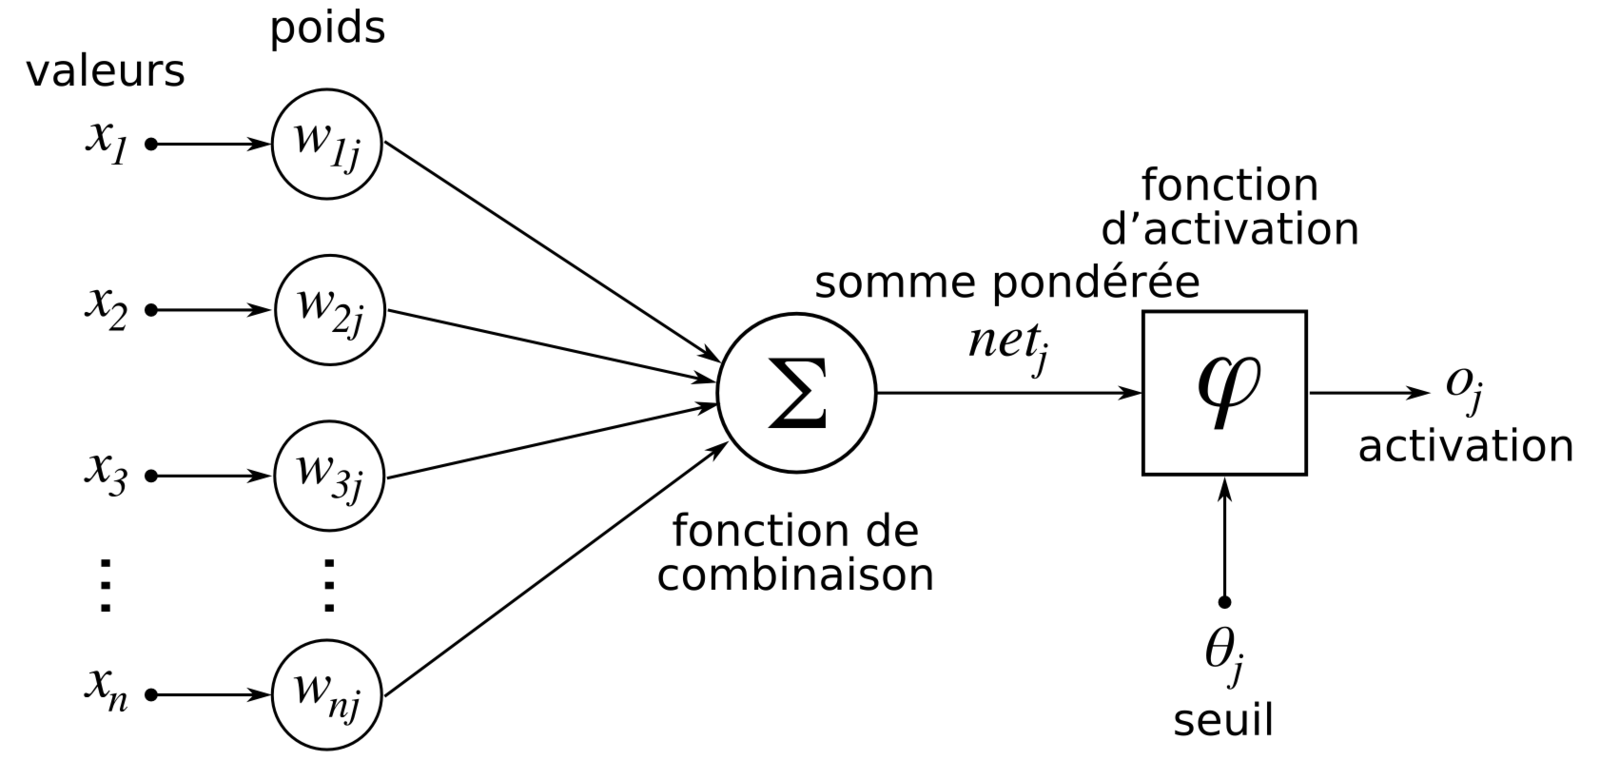
\includegraphics[width=10cm]{images_pfe/neurone.png}
	\caption{Le fonctionnement d'un neurone artificiel [\cite{mcculloch_pitts_1943_nervous_activity}].}
	\label{fig:fonctionnement-neurone}
\end{figure}
\FloatBarrier
\medskip

La fonction d'activation est utilisée pour introduire de la non-linéarité dans
le modèle, permettant ainsi de modéliser des relations complexes entre les
données d'entrée et de sortie [\cite{Goodfellow-et-al-2016}]. Les propriétés
d’une fonction d’activation doivent être vérifiées dans un problème
d'apprentissage profond. Ces propriétés sont:
\begin{itemize}
	\item \textbf{Non-linéarité}: lorsque la fonction d’activation est non linéaire, il est possible de prouver qu’un réseau neuronal à deux couches peut approximer n'importe quelle fonction continue sur un domaine compact à une précision arbitraire, ce que l’on appelle le \textbf{théorème d’approximation universelle} [\cite{Goodfellow-et-al-2016}].
	\item \textbf{L’intervalle}: lorsque l’intervalle des valeurs est fini, l'apprentissage de manière générale est plus efficace.
	\item \textbf{Différentiabilité}: cette propriété est importante quand les méthodes d’optimisation sont basées sur le gradient, car elles cherchent à optimiser l’apprentissage en se basant sur la  différentiabilité de la fonction.
	\item \textbf{Monotonie}: Une fonction d'activation est monotone si sa sortie augmente (ou diminue) à mesure que son entrée augmente. Cela garantit que le gradient de la fonction est toujours positif ou négatif, simplifiant ainsi l’apprentissage.
	\item \textbf{Efficacité en termes de calcul}: les fonctions d'activation doivent être efficaces en termes de calcul, afin que le réseau puisse être utilisé dans des applications en temps réel, sans ralentir le processus de l’apprentissage.
\end{itemize}
\medskip
Parmi les fonctions d'activation les plus couramment utilisées dans les réseaux de neurones, on peut citer:
\begin{itemize}
	\item \textbf{La fonction Sigmoïde}: si la probabilité d’un résultat est comprise entre 0 et 1, la fonction sigmoïde est le meilleur choix. Cette fonction est largement utilisée grâce à son intervalle et sa différentiabilité.
	      \begin{equation}
		      \sigma(x) = \frac{1}{1 + e^{-x}}
	      \end{equation}
	\item \textbf{La fonction Unité linéaire rectifiée (ReLU)}: c'est une fonction qui possède une dérivée et permet la rétropropagation (backpropagation) tout en étant efficace sur le plan informatique. Cependant, elle n’active pas les neurones en même temps, et c’est considéré comme désavantage pour cette fonction.
	      \begin{equation}
		      ReLU(x) = \max(0,x)
	      \end{equation}
	\item \textbf{La fonction Tangente hyperbolique (Tanh)}: cette fonction est très identique à la fonction d’activation sigmoïde. Sa plage de sortie est comprise entre -1 et 1. Avec cette fonction, plus l’entrée est grande, plus la valeur de sortie sera proche de 1, et plus l’entrée est petite, plus la sortie sera proche de -1.
	      \begin{equation}
		      tanh(x) = \frac{e^x - e^{-x}}{e^x + e^{-x}}
	      \end{equation}
\end{itemize}
\medskip
\begin{figure}[hbt!]
	\centering
	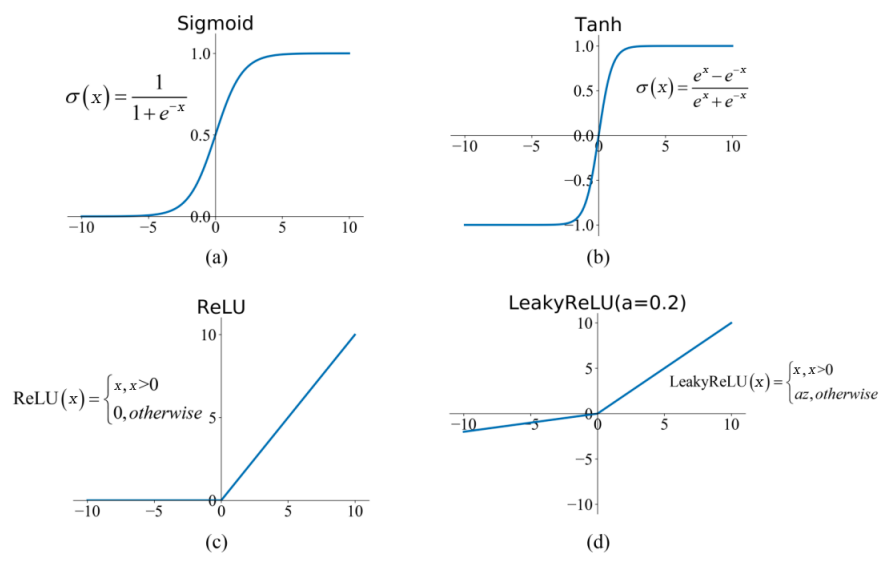
\includegraphics[width=12cm]{images_pfe/functions.png}
	\caption{Les fonctions d'activations couramment utilisées [\cite{feng_he_teng_ren_chen_li_2019}].}
	\label{fig:vue-snoc-pos}
\end{figure}
\FloatBarrier

\section{Couches dans un réseau de neurones}
Une couche (\textit{layer} en anglais) est une succession verticale des
neurones. Mathématiquement, elle est vue comme une composition de deux
fonctions \textit{h} et \textit{g} où \textit{g} est une fonction linéaire et
\textit{h} une fonction d’activation non linéaire. Cette composition de
fonction est définie par l'équation \ref{equ:couche}
[\cite{Goodfellow-et-al-2016}].

\begin{equation}
	y = h(g(x) + b)
	\label{equ:couche}
\end{equation}

\medskip
Une couche intermédiaire est donc l’ensemble des nœuds verticaux qui sont connectés à la couche précédente et à la couche suivante. La connectivité entre les couches détermine la manière dont les informations circulent sur le réseau. La façon de connexions des nœuds entre eux est différente d’une architecture à une autre [\cite{Goodfellow-et-al-2016}], et c’est ce qui détermine le type d'une couche:
\begin{itemize}
	\item \textbf{Couche entièrement connectée}: tous les neurones d'une couche sont connectés à tous les neurones de la couche suivante.
	\item \textbf{Couche partiellement connectée}: certains neurones ne sont pas connectés aux neurones de la couche suivante.
\end{itemize}

Les couches sont le composant principal des réseaux de neurones. Elles ont
plusieurs caractéristiques qui définissent leur comportement et influencent les
performances globales du réseau. Ces caractéristique sont les suivants:

\begin{itemize}
	\item \textbf{La matrice de poids}: Dans une couche d'un réseau de neurones, la matrice de poids est une matrice de paramètres qui représente les connexions entre les neurones d'entrée et les neurones de sortie de cette couche [\cite{aggarwal_2018}]. Elle définie la puissance des connexions entre les neurones des différentes couches. Chaque ligne de la matrice correspond aux poids associés à un neurone d'entrée particulier, et chaque colonne correspond aux poids associés à un neurone de sortie particulier,La taille de la matrice de poids dépend du nombre de neurones d'entrée et du nombre de neurones de sortie dans la couche.

	      La forme générale de la matrice de poids dans un réseau de neurones peut être
	      exprimée comme suit:
	      \begin{equation}
		      W = \begin{bmatrix}
			      w_{1,1} & w_{1,2} & ... & w_{1, m} \\
			      w_{2,1} & w_{2,2} & ... & w_{2, m} \\
			      ...     & ...     & ... & ...      \\
			      w_{n,1} & w_{n,2} & ... & w_{n, m}
		      \end{bmatrix}
	      \end{equation}

	      où $w_{i,j}$ représente le poids de la connexion entre le neurone \textit{i} de
	      la couche actuelle et le neurone \textit{j} de la couche suivante et
	      \textit{(n, m)} représente la dimension de la matrice.

	      La matrice de poids est crucial pour la performance du réseau neuronal,
	      puisqu'elle détermine la capacité du réseau d'apprendre et généraliser les
	      motifs a partir des données en entrées.

	\item \textbf{Type de couche}: Les couches forment les blocs de construction de base des réseaux de neurones. Elle permettent d'effectuer des calculs complexes et d'apprendre des relations qui existent entre données d'entrée et de sortie. Dans le réseau neuronal, il existe trois types de couches différents:
	      \begin{itemize}
		      \item \textbf{Couche d'entrée}: Cette couche est responsable de la réception des données d'entrée et de leur transmission à la couche suivante (la première couche parmi les couches cachées).
		      \item \textbf{Couche cachée}: Cette couche traite les entrées de la couche précédente et génère des valeurs de sortie qui sont transmises à la couche suivante. Les réseaux de neurones peuvent avoir plusieurs couches cachées, chacune effectuant différentes opérations sur les entrées.
		      \item \textbf{Couche de sortie}: Cette couche produit la sortie finale du réseau de neurones, qui peut être une classification, une régression ou un autre type de prédiction.
	      \end{itemize}
\end{itemize}

\medskip

\begin{figure}[hbt!]
	\centering
	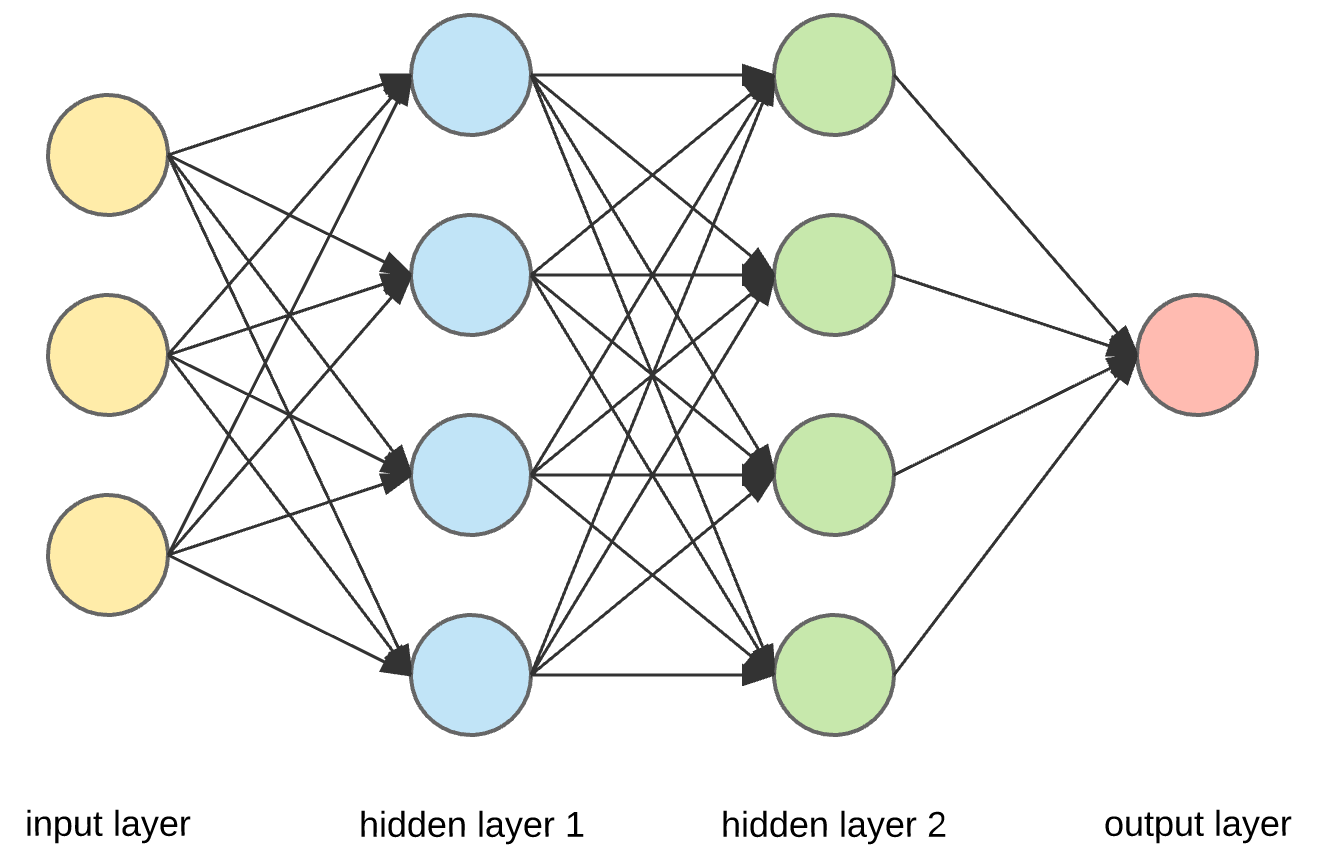
\includegraphics[width=12cm]{images_pfe/network.png}
	\caption{Schéma simple d'un réseau de neurones feedforward [\cite{dl-healthcare}].}
	\label{fig:schema-reseau}
\end{figure}
\FloatBarrier
\medskip

\section{Types de réseaux de neurones}
Dans l'apprentissage profond, il existe plusieurs classes de réseaux de
neurones, chacune avec sa propre architecture, caractéristiques, algorithme
d'apprentissage et application. Dans cette section, nous allons présenter les
différentes architecture de réseaux de neurones.
\subsection{Réseaux feedforward}
Les réseaux feedforward (ou réseaux entièrement connectés) sont un des types de
réseau de neurones artificiels où les informations circulent dans une seule
direction, de l'entrée vers la la sortie [\cite{Goodfellow-et-al-2016}]. Ils
sont composés d'une succession de couches interconnectées, où chaque neurone
d'une couche est connecté aux neurones de la couche suivante. Dans un Réseau de
ce type, les données sont introduites dans la première couche du réseau (couche
d'entrée), puis elles traversent plusieurs couches cachées avant d'atteindre la
couche de sortie (\textit{la figure \ref{fig:schema-reseau} est un schéma
	simple d'un réseau feedforward}).

Les réseaux feedforward sont indépendants de la structure, c’est-à-dire il
n’existe pas d’hypothèses particulières à faire sur l’entrée, ce qui les rend
largement applicables. Cependant, ils ont tendance à être moins performants que
les réseaux à usage spécial. Les réseaux feedforward sont couramment utilisés
dans les applications d'apprentissage supervisé. Ils peuvent également être
utilisés dans des applications d'apprentissage non supervisé
[\cite{aggarwal_2018}].

\medskip

\subsection{Réseaux de neurones récurrents (RNN)}
Les réseaux de neurones récurrents (RNN) sont des architectures conçus pour
fonctionner avec des données séquentielles, telles que: la reconnaissance de la
parole, la reconnaissance de la voie, l'analyse de séries chronologiques et le
traitement du langage naturel [\cite{Goodfellow-et-al-2016}]. Les principales
caractéristiques des RNN sont:
\begin{itemize}
	\item \textbf{Connexions récurrentes} : Les connexions dans les réseaux récurrents sont des connexions récurrentes qui permettent à l'information de persister au fil du temps. Cela signifie que la sortie du réseau à un pas de temps est réinjectée en entrée du réseau au pas de temps suivant.
	\item \textbf{État caché} : Les réseaux RNN maintiennent un état caché qui représente la mémoire du réseau. Cet état est mis à jour à chaque pas de temps en fonction de l'entrée courante et de l'état caché précédent.
	\item \textbf{RNN bidirectionnels} : Les réseaux RNN bidirectionnels traitent la séquence d'entrée dans les sens avant et arrière, ce qui permet de capturer le contexte des pas de temps passés et futurs.
\end{itemize}

\begin{figure}[hbt!]
	\centering
	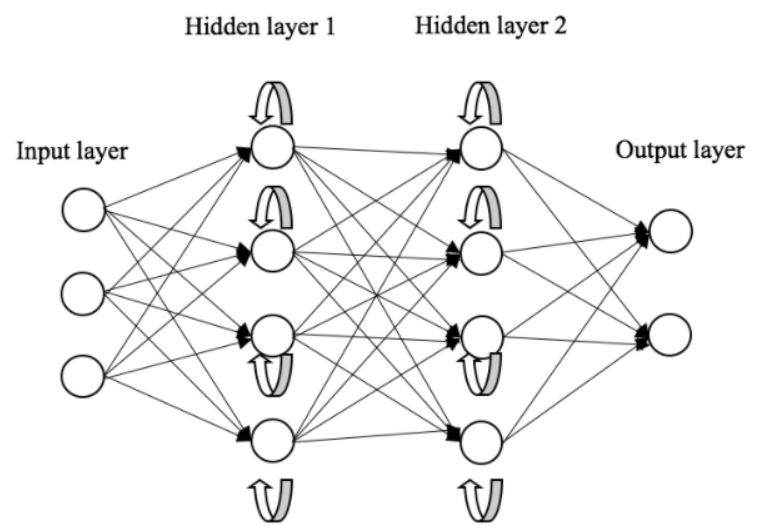
\includegraphics[width=12cm]{images_pfe/rnn.png}
	\caption{Exemple d'un réseau de neurones récurrent [\cite{kumaraswamy_2021}].}
	\label{fig:schema-reseau}
\end{figure}
\FloatBarrier

La capacité à conserver une mémoire des pas de temps précédents et à gérer les
dépendances à long terme rend les réseaux récurrents utiles pour les tâches qui
nécessitent de comprendre le contexte de la séquence d'entrée.

\subsubsection{Réseaux récurrents à mémoire courtet long terme (LSTM) }

Les réseaux de neurones récurrents à mémoire longue à court terme, ou Long
Short-Term Memory (LSTM) en angalis , représentent une amélioration
significative des réseaux de neurones récurrents traditionnels, conçue pour
résoudre les problèmes d’évanouissement et d’explosion du gradient. Introduits
par Hochreiter et Schmidhuber en 1997 dans [\cite{hochreiter1997long}], les
réseaux LSTM intègrent des cellules mémoire capables

de stocker et de conserver des informations tout au long du traitement d’une
séquence. Ces cellules mémoire permettent de transporter des informations
importantes grâce à trois types de portes : la porte d’entrée, la porte de
sortie et la porte d’oubli. Ces portes jouent un rôle crucial en décidant
quelles informations doivent être ajoutées, conservées ou oubliées.

\textbf{Porte d'Entrée}: décide quelles nouvelles informations doivent être stockées dans la cellule de mémoire. Elle est définie par :

\begin{equation}
	i_t = \sigma(W_i \cdot [h_{t-1}, x_t] + b_i)
\end{equation}

où $\sigma$ représente la fonction sigmoïde, $W_i$ est le poids associé à la
porte d'entrée, $h_{t-1}$ est l'état caché précédent, $x_t$ est l'entrée
actuelle, et $b_i$ est le biais.

\textbf{Porte d'Oubli}: contrôle quelles informations anciennes doivent être effacées de la cellule de mémoire. Elle est définie par :

\begin{equation}
	f_t = \sigma(W_f \cdot [h_{t-1}, x_t] + b_f)
\end{equation}

où $\sigma$ est la fonction sigmoïde, $W_f$ est le poids associé à la porte
d'oubli, $h_{t-1}$ est l'état caché précédent, $x_t$ est l'entrée actuelle, et
$b_f$ est le biais.

\textbf{Porte de Sortie}: décide quelles informations de la cellule de mémoire sont utilisées pour calculer l'état caché actuel. Elle est définie par :

\begin{equation}
	o_t = \sigma(W_o \cdot [h_{t-1}, x_t] + b_o)
\end{equation}

où $\sigma$ est la fonction sigmoïde, $W_o$ est le poids associé à la porte de
sortie, $h_{t-1}$ est l'état caché précédent, $x_t$ est l'entrée actuelle, et
$b_o$ est le biais.

\begin{figure}[hbt!]
	\centering
	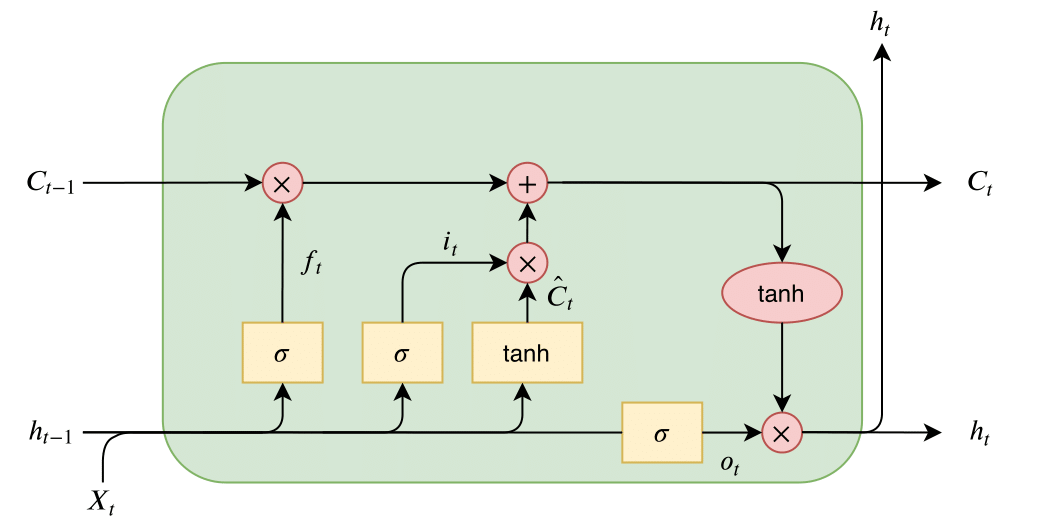
\includegraphics[width=15cm]{images_pfe/lstm.png}
	\caption{Architecture d'un bloc LSTM [\cite{fawaz2019long}].}
	\label{fig:lstm}
\end{figure}
\FloatBarrier
\medskip

\subsection{Réseaux de neurones convolutifs (CNN)}
L'architecture des réseaus de neurones convolutifs (CNN) est une architecture
spéciale qui est bien adaptée à la tâche de classification d'images. Ces
réseaux comportent trois types de couches: \textbf{convolutives},
\textbf{pooling} et \textbf{d'activation} [\cite{Goodfellow-et-al-2016}].

Les couches convolutives sont appliquées à l'image en entrée pour l’extraction
des caractéristiques importantes de l'image. Ensuite, ces dernières traversent
des couches d'activation, qui sont responsables de l'application d'une fonction
d'activation non-linéaire à ces caractéristiques. Les couches d'activation sont
suivies de couches de pooling qui réduisent la taille de l'image. Les couches
de pooling sont elles même suivies par une couche entièrement connectée qui
donne la classification de l'image (la sortie finale du modèle)
[\cite{Goodfellow-et-al-2016}].

\begin{figure}[hbt!]
	\centering
	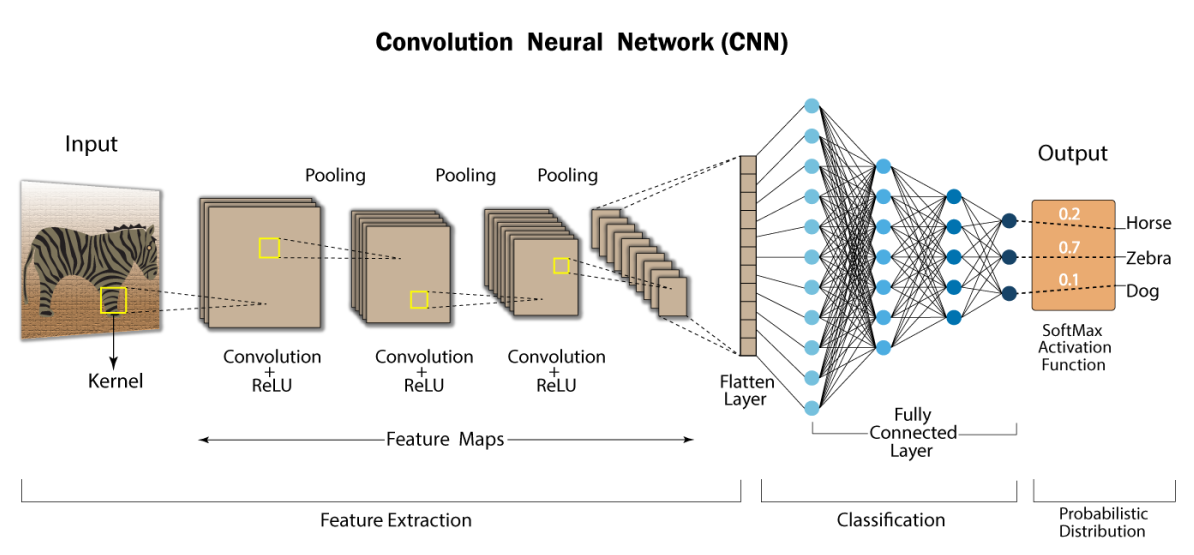
\includegraphics[width=15
		cm]{images_pfe/cnn.png}
	\caption{Le fonctionnement d'un réseau neuronal convolutif [\cite{alharbi_hewahi_2021}].}
	\label{fig:cnn}
\end{figure}
\FloatBarrier
\medskip

\subsubsection{Couche convolutive}
Une couche convolutive est un élément constitutif des réseaux de neurones
convolutifs (CNN). Elle est utilisé pour extraire des caractéristiques à partir
de données d'entrée, souvent des images, en appliquant un ensemble de filtres
convolutifs appris à l'entrée.

\medskip
Dans une couche convolutive, chaque filtre est convolué avec l'entrée pour produire une carte de caractéristiques. Cette opération est faite en glissant le filtre sur l'entrée et en calculant le produit scalaire à chaque position. Généralement, une couche convolutive possède trois hyperparamètres qui doivent être définis : \textbf{le nombre de filtres}, \textbf{la taille des filtres} et \textbf{la Stride}. Le nombre de filtres détermine le nombre de cartes d'entités produites, tandis que la taille des filtres détermine la taille du champ récepteur de chaque carte d'entités. La stride détermine la quantité de décalage du filtre à chaque étape.

\medskip
Les couches convolutives sont suivies de fonctions d'activation,et de couches de pooling. Ces dernières permettent de réduire les dimensions spatiales des cartes d'entités. Plusieurs couches convolutives peuvent être empilées pour créer un réseau neuronal convolutif profond.Les couches convolutives sont particulièrement efficaces pour traiter des images et d'autres données de grande dimension avec une structure spatiale, car elles peuvent apprendre automatiquement à détecter les caractéristiques importantes, telles que les bords, les coins et les textures [\cite{kimura_yoshinaga_sekijima_azechi_baba_2019}, \cite{Goodfellow-et-al-2016}].

\begin{figure}[hbt!]
	\centering
	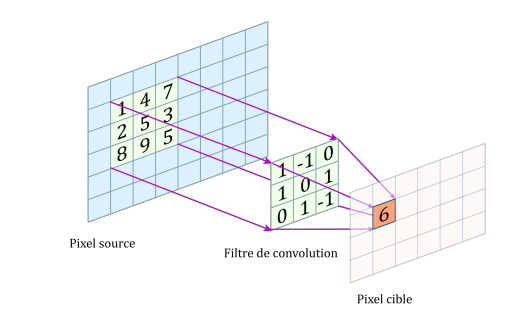
\includegraphics[width=12
		cm]{images_pfe/layerconv.png}
	\caption{Exemple du fonctionnement d'une couche convolutive [\cite{kimura_yoshinaga_sekijima_azechi_baba_2019}].}
	\label{fig:conv}
\end{figure}
\FloatBarrier
\medskip

\subsection{Réseaux résiduels (ResNet)}
Les réseaux résiduels ont été conçus par Microsoft afin de résoudre le problème
des gradients qui disparaissent dans les réseaux de neurones très profonds, ce
qui peut rendre l'entraînement difficile et diminuer significativement les
performances du réseau.

\medskip
Un ResNet est composé d'une ensemble de blocs résiduels, qui sont constitués de plusieurs couches avec des connexions de raccourci qui contournent une ou plusieurs couches. Ces raccourcis permettent aux gradients de circuler plus facilement à travers le réseau et évitent qu'ils ne disparaissent à mesure que le réseau devient plus profond [\cite{He_2016_CVPR}].

\begin{figure}[hbt!]
	\centering
	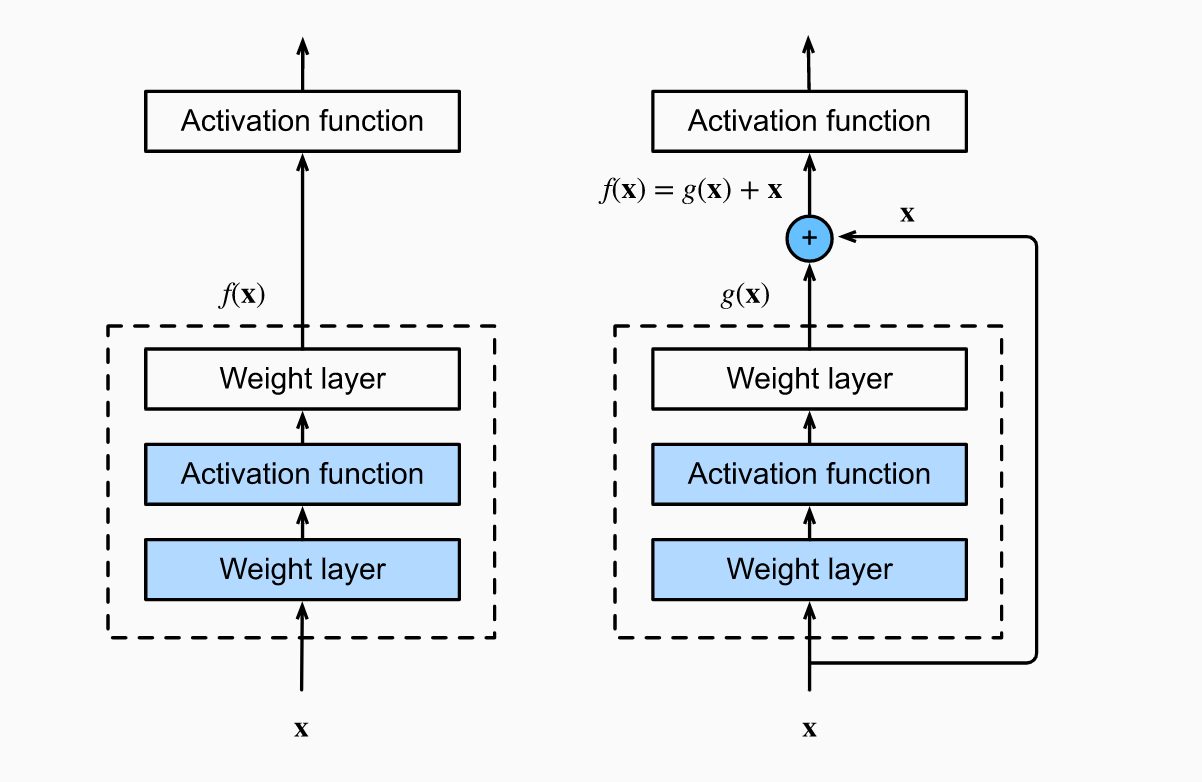
\includegraphics[width=12cm]{images_pfe/residual-net.png}
	\caption{Un bloc régulier (gauche) et un bloc résiduel (droite) [\cite{dong_niu_li_xie_zou_ye_wei_pan_2022}].}
	\label{fig:residual-net}
\end{figure}
\FloatBarrier

\medskip
ResNet est très efficace dans les tâches de vision par ordinateur, telles que la classification d'images, la détection d'objets et la segmentation. Il a joué un rôle important dans l'avancement de l'état de l'art en apprentissage profond et en vision par ordinateur, et continue d'être un domaine de recherche actif.

\section{Le processus d’apprentissage}
L’apprentissage est le processus itératif et continu d’ajustement des
paramètres du réseau neuronal afin d’obtenir une meilleure précision du modèle
[\cite{Goodfellow-et-al-2016}]. Il peut être complexe car il nécessite souvent
une combinaison de techniques telles que le \textbf{prétraitement} des données,
le choix de l'architecture du réseau de neurones et des hyperparamètres, ainsi
que l'algorithme d'optimisation.

Ce processus d'apprentissage commence d'abord par l'initialisation aléatoire
des paramètres (poids) du modèle. Ensuite, le modèle est entraîné sur un
ensemble de données (\textbf{dataset}) en utilisant un algorithme
d'optimisation pour ajuster les poids du modèle afin de minimiser la perte.

Lors de l'entraînement, le modèle est alimenté en entrée avec des exemples à
partir du dataset d'entrainement et compare sa sortie à la sortie attendue.
Ensuite, il calcul la perte en faisant la différence entre la sortie prédite et
la sortie attendue. L'algorithme de \textbf{rétropropagation} de gradient
ajuste les poids du modèle en claculant les gradient de la fonction de perte
afin de la minimiser.

Le processus d'apprentissage continue jusqu'à ce que la performance du modèle
sur le dataset de validation arrête de s'améliorer ou jusqu'à ce qu'un nombre
prédéfini d'itérations d'apprentissage soit atteint. Le modèle final est
ensuite utilisé pour effectuer des prédictions sur de nouvelles données.

\medskip
Ce processus peut être résumé dans les points suivants:
\begin{itemize}
	\item L’apprentissage consiste à modifier progressivement les paramètres (poids) en
	      passant un lot de données en entrée et en évaluant le taux de perte.
	\item La définition de la fonction de perte est utilisée pour les modifications de
	      réseaux dans le processus de l'entraînement.
	\item La modification des poids du réseau est effectuée grâce a l’algorithme de
	      rétropropagation (backpropagation).
\end{itemize}

\subsection{Descente de gradient}
La descente de gradient est une méthode utilisée dans le processus
d’optimisation. Elle est basée sur la différentiabilité d’une fonction et elle
est appliquée pour calculer la fonction dérivée du premier ordre pour trouver
le minimum de la fonction de perte [\cite{Goodfellow-et-al-2016}]. Sa
simplicité d’application est l’un des avantages de cette méthode.

L'algorithme commence par l'initialisation aléatoire des paramètres (poids) du
modèle. Ensuite, il calcule le gradient de la fonction de perte par rapport à
chaque paramètre. Le gradient indique la direction dans laquelle la fonction de
perte augmente le plus, donc l'algorithme met à jour les paramètres dans la
direction opposée au gradient pour réduire la valeur de perte. Ce processus est
répété itérativement jusqu'à ce que la valeur de perte ne puisse plus être
réduite ou jusqu'à ce qu'un critère d'arrêt soit atteint. Le taux
d'apprentissage est un hyperparamètre qui contrôle la taille des mises à jour
de paramètres et la vitesse de convergence de l'algorithme
[\cite{Goodfellow-et-al-2016}].

Des variantes de la descente de gradient existent, telles que la descente de
gradient stochastique, Adam et la descente de gradient avec moment.

\subsection{Propagation de l’erreur}
La propagation d'erreur est utilisée dans le processus d'apprentissage pour
calculer le gradient de la fonction de perte par rapport aux paramètres du
modèle [\cite{Goodfellow-et-al-2016}].

Dans la propagation d'erreur, l'erreur est propagée en arrière à travers les
couches du modèle, en commençant par la couche de sortie et en allant vers
l'entrée. Chaque couche calcule la dérivée de sa sortie par rapport à ses
entrées, qui est ensuite multipliée par l'erreur propagée de la couche
suivante. Ce processus est répété jusqu'à ce que l'erreur soit propagée jusqu'à
la couche d'entrée, où le gradient de la fonction de perte par rapport aux
paramètres du modèle est obtenu [\cite{Goodfellow-et-al-2016}].

\begin{figure}[hbt!]
	\centering
	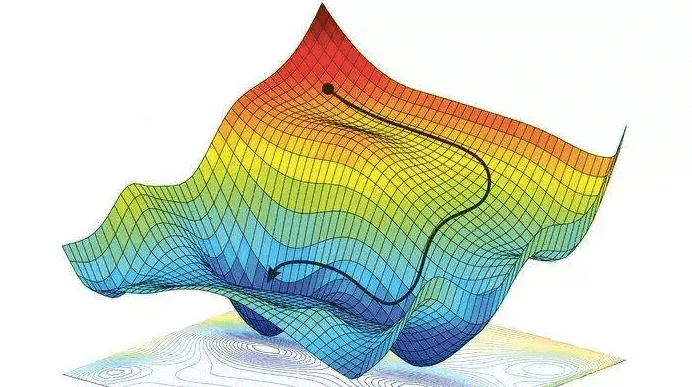
\includegraphics[width=10cm]{images_pfe/gd.png}
	\caption{Fonction de taux d’erreur [\cite{amini2018spatial}].}
	\label{fig:error-function}
\end{figure}
\FloatBarrier
\medskip

\subsection{Hyperparameters}
Les hyperparamètres sont les paramètres qui sont définis avant de lancer le
processus d'apprentissage et ils contrôlent l'entraînement. Les valeurs des
hyperparamètres, contrairement aux paramètres du modèle, ne sont pas apprises
lors de l'apprentissage [\cite{Goodfellow-et-al-2016}]. Parmi les
hyperparamètres, on peut définir:
\begin{itemize}
	\item \textbf{Taux d'apprentissage} : Il contrôle la vitesse d'apprentissage du modèle à partir des données.
	\item \textbf{Nombre d'époques} : Le nombre d'époques correspond au nombre d'itération sur le dataset d'entraînement.
	\item \textbf{Taille du batch} : Elle représente le nombre d'échantillons des données d'entraînement qui sont utilisés dans un passage avant/arrière (feedforward et backpropagation).
	\item \textbf{Nombre de couches} : C'est un hyperparamètre qui caractérise la profondeur du réseau.
	\item \textbf{Fonction d'activation} : La fonction d'activation est utilisée pour introduire la non-linéarité dans le modèle. C'est un hyperparamètre qui contrôle la sortie du neurone.
	\item \textbf{Initialisation des poids} : Les valeurs initiales des poids peuvent affecter de manière significative les performances du modèle. Elle affecte le processus de trouver le minimum local ou le minimum global.
	\item \textbf{Paramètre de régularisation} : Il est utilisé pour éviter le \textbf{surapprentissage}, c'est-à-dire éviter de construire un modèle qui est trop complexe par rapport à la quantité de données d'entraînement. Cela peut entraîner une adaptation excessive du modèle aux données d'entraînement et une mauvaise généralisation aux données inconnues.
	\item \textbf{Optimiseur} : L'optimiseur est l'algorithme utilisé pour mettre à jour les poids pendant l'entraînement.
\end{itemize}

Cependant, le réglage de ces hyperparamètres peut être une tâche complexe
nécessitant souvent des essais et des erreurs.

\section{Types d’apprentissage}
Il existe plusieurs types d’apprentissage, et chacun de ces types a des
applications spécifiques en deep learning, et peut être utilisé pour résoudre
différents types de problèmes. Dans ce qui suit, nous parlons brièvement sur
les quatre types d'apprentissage en deep learning les plus courants:
l'apprentissage supervisé, l'apprentissage non supervisé, l'apprentissage
semi-supervisé et l'apprentissage par renforcement.

\subsection{Apprentissage supervisé}
Dans l'apprentissage supervisé, l'apprentissage s'effectue sur un ensemble de
données étiqueté, où les étiquettes sont connues à l'avance. En d'autres
termes, les données d'entrée sont accompagnées d'étiquettes de sortie ou de
valeurs cibles correspondantes. Le but de l'apprentissage supervisé est
d'apprendre à prédire les étiquettes à partir des données d'entrée, de sorte
que lorsqu'on donne au modèle de nouvelles données en entrée, l'algorithme
puisse prédire la sortie correspondante. Pendant le processus d'apprentissage,
l'algorithme ajuste itérativement ses paramètres pour minimiser la différence
entre la sortie prédite et la sortie réelle [\cite{aggarwal_2018},
\cite{Goodfellow-et-al-2016}].

\medskip
Ce type d'apprentissage est applicable dans plusieurs domaines, tels que la reconnaissance d'images et de la parole, le traitement du langage naturel et la modélisation prédictive dans la finance, la santé, le marketing, etc. Parmi les algorithmes d'apprentissage supervisés, nous pouvons citer la régression linéaire et les arbres de décision.

\subsection{Apprentissage non-supervisé}
L'apprentissage non supervisé se fait sur un dataset non étiqueté, sans aucune
information sur les étiquettes [\cite{Goodfellow-et-al-2016}]. En d'autres
termes, il n'y a pas de valeurs cibles ou d'étiquettes de sortie fournies à
l'algorithme. L'algorithme est laissé à lui-même pour trouver les motifs et
relations dans les données, sans recevoir d'instructions explicites sur ce
qu'il faut rechercher.

\medskip
L'utilisation de cette approche d'apprentissage peut impliquer le regroupement de points de données similaires, la découverte de structures ou de caractéristiques cachées dans les données (réduction de la dimensionnalité) ou l'identification de valeurs aberrantes ou d'anomalies dans les données.

\medskip
Nous pouvons appliquer l'apprentissage non supervisé dans divers domaines, tels que la segmentation des marchés, la détection d'anomalies et l'extraction de caractéristiques. Parmi les algorithmes d'apprentissage non supervisés courants, on trouve le clustering k-means, l'analyse en composantes principales (PCA) et les auto-encodeurs.

\medskip
L'un des principaux défis dans l'apprentissage non supervisé est d'évaluer la qualité des résultats, car il n'y a pas d'objectifs ou d'étiquettes explicites à comparer. Au lieu de cela, les résultats sont souvent évalués en fonction de leur utilité ou de leur interprétabilité pour une tâche ou un domaine particulier.

\subsection{Apprentissage semi-supervisé}
L'apprentissage semi-supervisé est un type d'apprentissage qui combine des
éléments d'apprentissage supervisé et non supervisé. Dans l'apprentissage
semi-supervisé, un petit ensemble de données étiquetées est fourni, tandis que
la grande partie de données est non étiquetées [\cite{Goodfellow-et-al-2016}].

\medskip
Le but dans l'apprentissage semi-supervisé est d'utiliser les données étiquetées pour guider le processus d'apprentissage sur les données non étiquetées, afin d'améliorer la précision du modèle. Cela peut être particulièrement utile dans les situations où il est difficile ou coûteux d'obtenir des données étiquetées, mais il existe une abondance de données non étiquetées disponibles.

\medskip
Il existe plusieurs approches, mais une méthode courante consiste à utiliser les données étiquetées pour créer un modèle, puis à utiliser ce modèle pour faire des prédictions sur les données non étiquetées. Les étiquettes prédites sont ensuite utilisées pour améliorer le modèle, et le processus est répété de manière itérative.

\medskip
L'un des défis de l'apprentissage semi-supervisé est que la qualité des résultats peut dépendre fortement de la distribution des données non étiquetées. Si les données non étiquetées ne sont pas représentatives du domaine cible, le modèle peut mal fonctionner même avec une grande quantité de données non étiquetées.

\subsection{Apprentissage par renforcement}
L'apprentissage par renforcement se concentre sur la prise de décision. Il
s'agit d'une méthode d'apprentissage dans laquelle un agent apprend à prendre
des décisions en interagissant avec un environnement. L'agent doit choisir une
action à partir d'un état donné, et l'environnement renvoie un signal de
récompense ou de pénalité en fonction de l'action choisie. L'objectif de
l'agent est de maximiser la récompense totale sur une période donnée
[\cite{wiering2012reinforcement}]. Dans le chapitre suivant, nous présenterons
l'apprentissage par renforcement et nous en parlerons avec plus de détails.

\section{Catégories de données}
La division du jeu de données est une étape cruciale avant de commencer
l'entraînement du modèle de manière. Elle permet d'éviter les problèmes de
surapprentissage. Il est courant de diviser un jeu de données en trois parties
distinctes: l'ensemble d'entraînement, l'ensemble de validation et l'ensemble
de test [\cite{Goodfellow-et-al-2016}].

\begin{itemize}
	\item \textbf{Ensemble d'entraînement}: Il s'agit de la partie de données utilisée pour entraîner le modèle. Il est important que ce dataset soit représentatif de l'ensemble des données et qu'il contienne une variété de cas d'utilisation différents.

	\item \textbf{Ensemble de validation}: Il s'agit d'un sous-ensemble de l'ensemble de données utilisé pour évaluer les performances du modèle pendant l'entraînement. L'ensemble de validation est utilisé pour régler les hyperparamètres du modèle et pour éviter le surapprentissage. Il est important qu'il soit représentatif et distinct du dataset d'entraînement.

	\item \textbf{Ensemble de test}: Il s'agit d'un ensemble de données utilisé pour évaluer les performances du modèle après son entraînement. L'ensemble de test est utilisé pour obtenir une estimation impartiale de la performance du modèle sur de nouvelles données inédites, donc il est nécessaire que ce dataset soit représentatif de l'ensemble des données et distinct des deux autres datasets cités précédemment.
\end{itemize}
La distinctivité des datasets assure que le modèle se généralise bien aux nouvelles données invisibles. En règle générale, l'ensemble de données est divisé en ces trois ensembles dans un rapport de 60-20-20 ou 70-15-15 respectivement.

\section{Défis de l'apprentissage profond}
L'apprentissage profond a fait des progrès remarquables ces dernières années et
a obtenu des résultats excellents dans divers domaines tels que la vision par
ordinateur, le traitement du langage naturel et la reconnaissance de la parole.
Cependant, il reste encore plusieurs défis à relever afin d'améliorer encore
l'efficacité et l'efficience des modèles d'apprentissage profond. Certains
défis majeurs incluent:
\begin{itemize}
	\item \textbf{Rareté des données} : les modèles d'apprentissage profond nécessitent une grande quantité de données pour être entraînés efficacement. Cependant, dans de nombreux domaines, tels que l'imagerie médicale et la conduite autonome, les données sont rares et coûteuses à collecter.

	\item \textbf{Surapprentissage (overfitting)} : les modèles d'apprentissage profond peuvent facilement sur-adapter les données d'apprentissage, en particulier lorsque le modèle comporte un grand nombre de paramètres. Le surapprentissage peut entraîner de mauvaises performances de généralisation sur de nouvelles données.

	\item \textbf{Interprétabilité} : les modèles d'apprentissage profond sont souvent appelés "boîtes noires" car il peut être difficile de comprendre comment ils arrivent à leurs prédictions. Ce manque d'interprétabilité peut compliquer le débogage et l'amélioration des modèles de l’apprentissage profond

	\item \textbf{Limitations matérielles} : les modèles d'apprentissage profond  sont coûteux en termes de calcul et nécessitent un matériel spécialisé tel que des unités de traitement graphique (GPU) ou des unités de traitement de tenseur (TPU). Le coût de ce matériel peut constituer un obstacle pour les petits groupes de chercheurs ou les entreprises.

	\item \textbf{Attaques contradictoires} : les modèles d'apprentissage profond  peuvent être vulnérables aux attaques contradictoires, où un attaquant manipule délibérément les données d'entrée pour amener le modèle à faire des prédictions incorrectes.

\end{itemize}

\section{Conclusion}
En conclusion, l'apprentissage profond est devenu un domaine de recherche actif
de l'apprentissage automatique qui a révolutionné la façon dont nous abordons
de nombreux problèmes difficiles, tels que la vision par ordinateur, le
traitement du langage naturel et la robotique. Avec l'avènement d'un matériel
puissant, d'ensembles de données à grande échelle et d'algorithmes
sophistiqués, les modèles d'apprentissage profond ont connu un avancement
remarquable dans plusieurs domaines tels que la reconnaissance d'images, la
reconnaissance vocale, la traduction linguistique et la conduite autonome.

\medskip
Malgré son énorme succès, l'apprentissage en profondeur fait encore face à plusieurs défis, tels que le besoin d'algorithmes d'entraînement plus efficaces et fiables, une meilleure interprétabilité, etc. L’utilisation et l'entraînement de modèles d’apprentissage profond exigent des ordinateurs assez puissants et ne peuvent pas être utilisés sur les appareils moins puissants comme les ordinateur embarqués ou les smartphones, ce qui signifie qu'on a besoin de trouver des moyens pour optimisation ces modèles afin de les utiliser ultérieurement par les machines moins puissantes. Ces méthodes d'optimisation font l'objet du dernier chapitre.

\medskip
Dans ce qui suit, nous présenterons l'apprentissage profond et ses algorithmes. La raison pour laquelle on a réservé un chapitre complet pour l'apprentissage profond est que ce type d'apprentissage peut aider beaucoup dans l'optimisation des réseaux de neurones profonds, comme nous le verrons plus tard.

\clearpage

%%%%%%%%%%%%%%%%%%%%%%%%%%%%%% Intelligence artificielle générative (GenAI) %%%%%%%%%%%%%%%%%%%%%%%%%%%%%%%%%%%%%%%

\chapter{Intelligence Artificielle Générative (GenAI)}
\section{Introduction}

Avec les avancées fulgurantes du deep learning, de nouvelles méthodes
d'intelligence artificielle ont émergé, souvent désignées sous le terme de
modèles génératifs. Ces technologies de pointe, telles que les auto-encodeurs
variationnels (VAE), les réseaux adversariaux génératifs (GANs), les modèles de
diffusion, les transformers et les modèles de langage de grande taille (LLM)
sont capables de produire des données d'une qualité impressionnante,
ressemblant de manière frappante aux données réelles. Les données générées par
ces modèles sont souvent indiscernables des données authentiques, ces modèles
génératifs permettent la génération de textes, d'images, de séries temporelles
et de données tabulaires avec une grande précision.

\medskip

Dans ce chapitre, nous allons examiner en détail les différentes architectures
de ces modèles génératifs, ainsi que les techniques et pratiques associées à
leur fonctionnement et à leur mise en œuvre. Nous aborderons les principes de
base, les innovations récentes, et les applications potentielles de ces
technologies révolutionnaires.

\section{Les Auto-Encodeurs Variationnels (VAE)}
\subsection{Introduction}

Les auto-encodeurs variationnels (VAE) sont des modèles génératifs puissants,
reconnus pour leur capacité à apprendre une représentation compacte et
structurée des données. Cette approche a révolutionné le domaine de
l'apprentissage non supervisé et des modèles génératifs. Les VAE appartiennent
à la classe des modèles génératifs probabilistes, combinant les principes des
autoencodeurs et des modèles de variational Bayes pour générer des données
nouvelles et similaires à celles d'un jeu de données d'entraînement. Depuis
leur introduction par Kingma et Welling en 2013
	[\cite{kingma_welling_auto_encoding}] , les VAE ont connu un grand succès dans
diverses applications, allant de la génération d'images à la synthèse de texte.

\subsection{Fonctionnement}
Les VAE sont composés de trois éléments principaux (Figure \ref{fig:VAE}):
l'encodeur, le décodeur et l'espace latent. Chacune de ces composantes joue un
rôle crucial dans le fonctionnement global du modèle.

\textbf{L'Encodeur:}L'encodeur est responsable de la transformation des données d'entrée \(\mathbf{x}\) en une distribution
dans l'espace latent. Plus précisément, il mappe les données d'entrée à une distribution gaussienne paramétrée par
une moyenne \(\mu\) et une variance \(\sigma^2\). Cette distribution est souvent représentée par la formule \ref{equ:Enc}:

\begin{equation}
	q(\mathbf{z} \mid \mathbf{x}) = \mathcal{N}(\mathbf{z} \mid \mu(\mathbf{x}), \sigma^2(\mathbf{x}))
	\label{equ:Enc}
\end{equation}

où \(\mathbf{z}\) est la variable latente que l'encodeur cherche à estimer.

\medskip

\textbf{Le Décodeur:}Le décodeur prend un échantillon \(\mathbf{z}\) de la distribution gaussienne dans
l'espace latent et génère une reconstruction \(\hat{\mathbf{x}}\) des données d'entrée. Il modélise la distribution
des données d'entrée conditionnellement à \(\mathbf{z}\), La distribution des données générées est souvent exprimée par la formule \ref{equ:Dec} :

\begin{equation}
	p(\mathbf{x} \mid \mathbf{z})
	\label{equ:Dec}
\end{equation}

Typiquement, le décodeur est un réseau neuronal qui produit les paramètres de
cette distribution, souvent supposée gaussienne ou Bernoulli selon la nature
des données.

\medskip

\textbf{L'Espace latent:}est la représentation comprimée et structurée des données d'entrée.
Il est généralement conçu comme un espace continu, où chaque point de l'espace latent correspond à une instance
possible de données générées. L'idée est que cet espace latent capture les caractéristiques essentielles
des données d'entrée de manière à permettre
la génération de nouvelles instances en échantillonnant de cet espace.

\begin{figure}[hbt!]
	\centering
	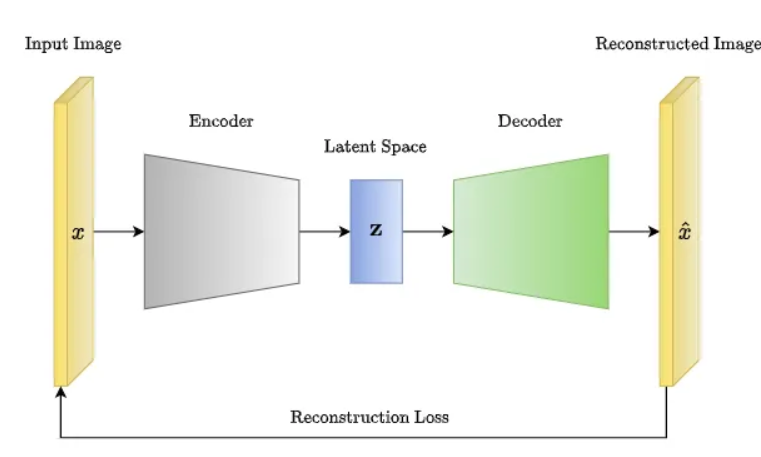
\includegraphics[width=10cm]{images_pfe/vae_1.png}
	\caption{Les composants d'un auto-encodeur variationnel (VAE)  [\cite{kingma_welling_auto_encoding}].}
	\label{fig:VAE}
\end{figure}

L’objectif principal d’un VAE est d’optimiser une fonction de coût qui combine
deux termes principaux : la divergence de Kullback-Leibler (KL)
[\cite{johnson2001symmetrizing}] et la vraisemblance de reconstruction.

\textbf{Divergence de Kullback-Leibler (KL)}: Ce terme mesure la différence entre la distribution latente approximée \( q(z | x) \) et la distribution prior \( p(z) \). La divergence KL est donnée par \ref{equ:KL} :

\begin{equation}
	D_{KL}(q(\mathbf{z} \mid \mathbf{x}) \parallel p(\mathbf{z}))
	\label{equ:KL}
\end{equation}

où \( q(z | x) \) est la distribution gaussienne paramétrée par l'encodeur, et
\( p(z) \) est généralement choisie comme une distribution normale standard.

\subsection*{Vraisemblance de Reconstruction}

Ce terme mesure la capacité du modèle à reconstruire les données d'entrée \( x
\) à partir de la variable latente \( z \). Il est donné par la vraisemblance
de \( x \) conditionnée par \( z \), La formule de vraisemblance de
reconstruction est exprimée dans l'équation \ref{equ:vr}:

\begin{equation}
	\log p(\mathbf{x} \mid \mathbf{z})
	\label{equ:vr}
\end{equation}

\subsubsection*{Fonction de Perte VAE}

La fonction de coût totale d'un VAE, également appelée fonction de perte VAE,
combine ces deux termes. L'équation de cette fonction de coût est donnée comme
suit \ref{equ:perte_vae} :
\begin{equation}
	\mathcal{L}(\theta, \phi; \mathbf{x}) = - \mathbb{E}_{q_\phi(\mathbf{z} \mid \mathbf{x})}[\log p_\theta(\mathbf{x} \mid \mathbf{z})] + D_{KL}(q_\phi(\mathbf{z} \mid \mathbf{x}) \parallel p(\mathbf{z}))
	\label{equ:perte_vae}
\end{equation}

où \( \theta \) et \( \phi \) sont les paramètres du décodeur et de l'encodeur
respectivement. Le premier terme, \( - \mathbb{E}_{q_\phi(z | x)}[\log
	p_\theta(x | z)] \), représente l'erreur de reconstruction, et le second terme,
\( D_{KL}(q_\phi(z | x) \parallel p(z)) \), régularise la distribution latente
pour qu'elle soit proche de la distribution prior.

En optimisant cette fonction de perte, les VAE parviennent à apprendre des
représentations latentes qui permettent une reconstruction fidèle des données
d'entrée tout en assurant une régularité statistique dans l'espace latent.

\subsection{Applications des Auto-Encodeurs Variationnels (VAE)}

Les auto-encodeurs variationnels (VAE) ont démontré leur efficacité dans divers
domaines grâce à leur capacité à apprendre des représentations latentes
significatives. Voici quelques-unes des principales applications des VAE :

\subsubsection{Génération d'Images}

Les VAE sont largement utilisés pour générer des images réalistes. En apprenant
une représentation latente des images d'entraînement, les VAE peuvent
échantillonner de cet espace latent pour créer de nouvelles images qui
partagent des caractéristiques similaires avec les données d'origine. Cela a
des applications potentielles dans la création de contenu, la conception
assistée par ordinateur et la synthèse d'images médicales
[\cite{luhman2024highfidelity}].

\subsubsection{Synthèse de Texte}

Les VAE peuvent être appliqués à la génération de texte en apprenant les
structures latentes des séquences de texte. Ils permettent de produire des
phrases cohérentes et des paragraphes qui imitent le style et le contenu des
textes d'entraînement. Cette technique est utile dans des domaines tels que la
génération automatique de rapports, l'écriture créative assistée et la
traduction automatique[\cite{wang2019topic}].

\subsubsection{Compression de Données}

Les VAE sont efficaces pour la compression de données, en particulier pour des
données de grande dimension comme les images et les vidéos. En apprenant une
représentation latente compacte, les VAE peuvent réduire la dimensionnalité des
données tout en préservant leurs caractéristiques essentielles. Cela permet une
transmission et un stockage plus efficaces des données
compressées[\cite{yilmaz2021selfvae}].

\subsubsection{Détection d'Anomalies}

Dans les systèmes de détection d'anomalies, les VAE peuvent être utilisés pour
identifier des données aberrantes qui diffèrent significativement des données
d'entraînement. En apprenant une distribution latente des données normales, le
VAE peut détecter des échantillons qui ne correspondent pas à cette
distribution, ce qui est particulièrement utile dans la surveillance de
systèmes industriels, la cybersécurité et la détection de fraudes
	[\cite{wang2019revisiting}].

\subsubsection{Imputation de Données Manquantes}

Les VAE peuvent également être employés pour l'imputation de données
manquantes. En apprenant la structure latente des données complètes, les VAE
peuvent estimer les valeurs manquantes de manière cohérente avec les données
observées. Cette application est cruciale dans des domaines tels que l'analyse
de données médicales, les études socio-économiques et les bases de données
incomplètes [\cite{collier2020vaes}].

En résumé, les VAE sont des outils polyvalents dans le domaine de
l'apprentissage machine, avec des applications variées allant de la génération
de contenu à la compression de données et à la détection d'anomalies. Leur
capacité à apprendre des représentations latentes significatives permet de
traiter efficacement une large gamme de problèmes complexes.

%%%%%%%%%%%%%%%%%%%%%%%%%%%%%%%%%%%%%%%%%%%%%%%%% Réseaux Antagonistes Génératifs (GANs) %%%%%%%%%%%%%%%%%%%%%%%%%%%%%%%%%%%%%%%%%%%%%%%%%
\section{Réseaux Antagonistes Génératifs (GANs)}

\subsection{Introduction aux Réseaux Antagonistes Génératifs}

Les réseaux antagonistes génératifs, ou Generative Adversarial Networks (GANs)
en anglais, sont une classe de modèles génératifs introduite par Ian Goodfellow
et ses collègues en 2014 [\cite{goodfellow2014generative}]. Les GANs se
composent de deux réseaux de neurones concurrents : un générateur et un
discriminateur. Le générateur cherche à produire des échantillons réalistes à
partir d'un bruit aléatoire, tandis que le discriminateur tente de distinguer
les échantillons réels des échantillons générés. Cette compétition incite les
deux réseaux à s'améliorer simultanément, aboutissant à la génération de
données de haute qualité.

\subsection{Fonctionnement des GANs}

Les GANs sont des modèles très performants et sont adaptés à plusieurs
architectures variées. Cependant, ils se composent principalement de deux
réseaux de neurones principaux :

\subsubsection{Générateur}

Le réseau générateur prend un vecteur de bruit \( z \) tiré d’une distribution
uniforme ou normale et produit une donnée synthétique \( G(z) \).
Mathématiquement, le générateur peut être représenté comme une fonction \( G :
Z \rightarrow X \), où \( Z \) est l'espace du bruit et \( X \) est l'espace
des données. L’objectif du générateur est de "tromper" le discriminateur en
générant des données indiscernables des données réelles, la fonction qui
représent le réseaux de neurones génerateur est donnée comme suite
\ref{equ:gen_gan}:

\begin{equation}
	G(\mathbf{z}; \theta_g) : \mathbf{z} \sim p_z(\mathbf{z}) \rightarrow \mathbf{x} = G(\mathbf{z})
	\label{equ:gen_gan}
\end{equation}

où \( \theta_g \) représente les paramètres du générateur, \( p_z(z) \) est la
distribution du bruit (généralement uniforme ou normale), et \( x \) est la
donnée synthétique générée.

Le générateur apprend à partir des erreurs du discriminateur, en améliorant
constamment la qualité des données générées. En d'autres termes, il essaie de
maximiser la probabilité que le discriminateur classifie ses sorties comme
étant des données réelles.

\subsubsection{Discriminateur}

Le réseau discriminateur reçoit soit une donnée réelle \( x \) soit une donnée
générée \( G(z) \). Il sort une probabilité \( D(x) \) ou \( D(G(z)) \)
indiquant si l’entrée est réelle ou générée. Mathématiquement, le
discriminateur peut être représenté comme une fonction \( D : X \rightarrow [0,
	1] \), où \( D(x) \) représente la probabilité que \( x \) soit une donnée
réelle, la fonction qui représent lé réseaux de neurones est donnée par
\ref{equ:dis_gan}:

\begin{equation}
	D(\mathbf{x}; \theta_d) : \mathbf{x} \rightarrow [0, 1]
	\label{equ:dis_gan}
\end{equation}

où \( \theta_d \) représente les paramètres du discriminateur.

Le discriminateur est entraîné pour maximiser la probabilité d’assigner la
bonne étiquette aux échantillons réels et générés. Il essaie de minimiser la
probabilité d'être trompé par les fausses données produites par le générateur.

Le discriminateur est, en essence, un classificateur binaire qui essaie de
distinguer entre les données authentiques et celles générées.

\subsubsection{Fonction de Perte}

Les fonctions de perte pour le discriminateur et le générateur sont définies
comme suit dans \ref{equ:gan_d_perte} et \ref{equ:gan_g_perte} respectivement :

\begin{equation}
	\mathcal{L}_D = -\mathbb{E}_{\mathbf{x} \sim p_{data}}[\log D(\mathbf{x})] - \mathbb{E}_{\mathbf{z} \sim p_z}[\log(1 - D(G(\mathbf{z})))]
	\label{equ:gan_d_perte}
\end{equation}

\begin{equation}
	\mathcal{L}_G = -\mathbb{E}_{\mathbf{z} \sim p_z}[\log D(G(\mathbf{z}))]
	\label{equ:gan_g_perte}
\end{equation}

Où :
\begin{conditions}
	\mathcal{L}_D & fonction de perte du discriminateur \\
	\mathcal{L}_G & fonction de perte du générateur \\
	x & donnée réelle tirée de la distribution \( p_{data} \) \\
	z & vecteur de bruit tiré de la distribution \( p_z \) \\
	D(x) & probabilité estimée par le discriminateur que \( x \) soit une donnée réelle \\
	G(z) & donnée synthétique générée à partir du bruit \( z \)
\end{conditions}

L'objectif du générateur est de minimiser \( \mathcal{L}_G \), tandis que le
discriminateur cherche à minimiser \( \mathcal{L}_D \). Plus formellement,
l'objectif est de résoudre le problème de minimax définit dans l'équation
\ref{equ:prob_gan} :

\begin{equation}
	\min_G \max_D \mathbb{E}_{\mathbf{x} \sim p_{data}}[\log D(\mathbf{x})] + \mathbb{E}_{\mathbf{z} \sim p_z}[\log(1 - D(G(\mathbf{z})))]
	\label{equ:prob_gan}
\end{equation}

\subsubsection{Entraînement des GANs}

L’entraînement des réseaux antagonistes génératifs (GANs) implique une série
d'étapes répétitives où le générateur et le discriminateur sont mis à jour tour
à tour pour améliorer leurs performances respectives. Le processus se déroule
comme suit :

L'entraînement des GANs se fait par les étapes suivantes :
\begin{enumerate}
	\item Tirer un échantillon de bruit \( z \) de la distribution \( p_z \).
	\item Générer une donnée synthétique \( G(z) \) à partir du générateur.
	\item Tirer un échantillon de données réelles \( x \) de la distribution de données
	      \( p_{data} \).
	\item Mettre à jour les poids du discriminateur \( D \) en minimisant la fonction de
	      perte \( \mathcal{L}_D \).
	\item Tirer un nouvel échantillon de bruit \( z \).
	\item Mettre à jour les poids du générateur \( G \) en minimisant la fonction de
	      perte \( \mathcal{L}_G \).
	\item Répéter les étapes ci-dessus pour un nombre prédéfini d'itérations.
\end{enumerate}

En suivant ces étapes, les GANs sont entraînés pour générer des données
synthétiques réalistes qui peuvent être utilisées dans diverses applications,
telles que la génération d'images, la super-résolution d'images et la synthèse
de texte.

\begin{figure}[hbt!]
	\centering
	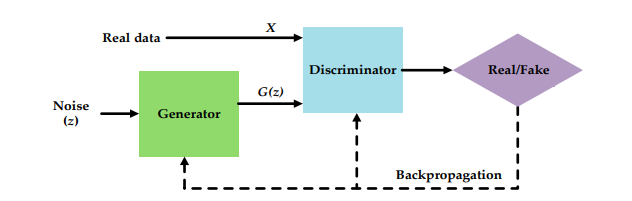
\includegraphics[width=12cm]{images_pfe/gan_1.png}
	\caption{Architecture du modèle de GANs [\cite{feng_feng_chen_cao_zhang_jiao_yu_2020}].}
	\label{fig:gan}
\end{figure}
\FloatBarrier

\subsection{Applications des GANs}

Les GANs ont une variété d'applications dans différents domaines :

\subsubsection{Génération d'Images}

Les GANs sont largement utilisés pour générer des images réalistes. Ils ont été
appliqués avec succès dans la création d'images de haute qualité, la génération
de visages humains, et même la création artistique. Par exemple, les GANs
peuvent générer des images de personnes qui n'existent pas en apprenant les
caractéristiques des visages humains à partir de vastes bases de données
d'images.

\subsubsection{Super-Résolution d'Images}

Les GANs sont également utilisés pour la super-résolution d'images,
c'est-à-dire augmenter la résolution d'une image basse résolution. Le modèle
SRGAN (Super-Resolution GAN) est un exemple où les GANs sont utilisés pour
produire des images de haute résolution à partir d'images de basse résolution,
améliorant ainsi les détails visuels et la clarté [\cite{ledig2017photo}].

\subsubsection{Synthèse de Texte et Traduction Automatique}

Dans le traitement du langage naturel (NLP), les GANs sont appliqués à la
génération de texte et à la traduction automatique [\cite{de2021survey}]. Les
modèles basés sur les GAN peuvent générer des phrases cohérentes et
contextuellement appropriées, imitant le style et le contenu des textes
d'entraînement. Cela est particulièrement utile pour les applications comme les
chatbots, la création de contenu textuel, et les systèmes de traduction.

\subsubsection{StyleGAN: This Person Does Not Exist}

StyleGAN, ou Style-Based Generator Architecture for Generative Adversarial
Networks, est un modèle génératif avancé développé par les chercheurs de
NVIDIA[\cite{karras2019style}]. Il représente une avancée significative dans la
génération d'images de haute qualité et photoréalistes, y compris les visages
de personnes qui n'existent pas. StyleGAN a diverses applications, y compris
dans l'industrie du divertissement, la réalité virtuelle et la recherche
académique.

\textbf{This Person Does Not Exist}: Un exemple frappant de l'application de StyleGAN est le site web "This Person Does Not Exist" [\cite{thispersondoesnotexist}]  . Ce site utilise un modèle StyleGAN pour générer de manière aléatoire des visages de personnes qui n'existent pas à chaque rechargement de la page.

\begin{figure}[hbt!]
	\centering
	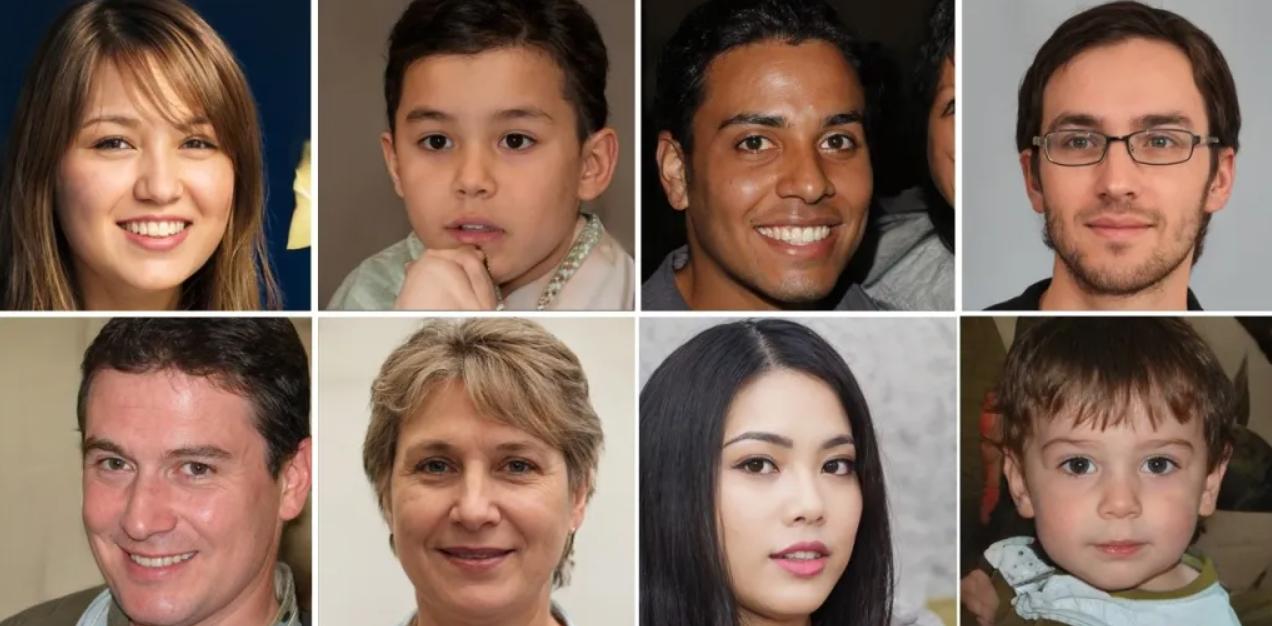
\includegraphics[width=12cm]{images_pfe/thisperson.png}
	\caption{Quelques images générées par le modèle StyleGAN sur le site 'This Person Does Not Exist'[\cite{thispersondoesnotexist}].}
	\label{fig:thisperson}
\end{figure}
\FloatBarrier

En résumé, les GANs sont des outils puissants et polyvalents dans le domaine de
l'apprentissage machine, avec des applications qui vont de la génération
d'images à la traduction automatique. Leur capacité à apprendre et à générer
des données réalistes ouvre de nombreuses perspectives dans divers domaines.

%%%%%%%%%%%%%%%%%%%%%%%%%%%%%%%%%%Diffusion Model%%%%%%%%%%%%%%%%%%%%%%%%%%%%%%%%%%%%
\section{Diffusion models}
\subsection{Introduction}

Les modèles de diffusion, également connus sous le nom de diffusion models en
angalais, représentent une avancée significative dans le domaine des modèles
génératifs au sein de l'apprentissage automatique. Émergents de manière
proéminente ces dernières années, ces modèles ont attiré l'attention pour leur
remarquable capacité à générer des données synthétiques de haute qualité, les
positionnant comme une alternative prometteuse aux techniques plus établies
telles que les Réseaux Antagonistes Génératifs (GANs) et les Autoencodeurs
Variationnels (VAEs) [\cite{dhariwal2021diffusion}].

La fondation conceptuelle des modèles de diffusion s'inspire des processus de
diffusion physique, où les particules migrent des régions de haute
concentration vers des zones de moindre concentration [\cite{ho2020denoising}]
. Ces modèles sont également basés sur les chaînes de Markov comme illustré
dans la figure \ref{fig:markov}, un concept clé en probabilité qui décrit une
série de transitions d'état où chaque état dépend uniquement de l'état
précédent. Dans le contexte des données, ce principe est exploité pour affiner
progressivement les données bruitées en représentations réalistes
[\cite{yang2022diffusion}].

\begin{figure}[hbt!]
	\centering
	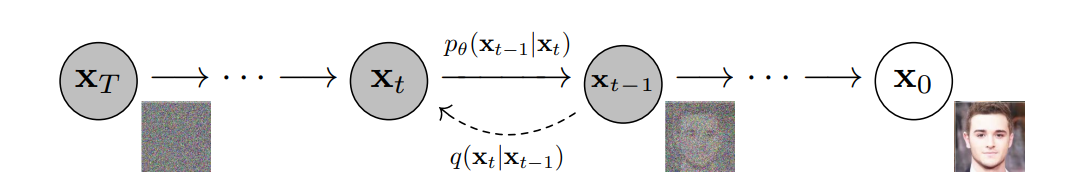
\includegraphics[width=12cm]{images_pfe/markov.png}
	\caption{Chaîne de Markov du processus de diffusion [\cite{ho2020denoising}].}
	\label{fig:markov}
\end{figure}
\FloatBarrier

\subsection{Fonctionnement des Modèles de Diffusion}

Les modèles de diffusion utilisent un processus en deux étapes cruciale[Figure
		\ref{fig:pro_diff}] : le bruitage (noising en anglais, également appelé Forward
Process) et le débruitage (denoising en anglais, ou Reverse Process). Ces
étapes sont essentielles pour transformer des données réelles en une
distribution de bruit et inversement. Le Forward Process consiste à ajouter
progressivement du bruit aux données réelles, les transformant ainsi en une
séquence de données de plus en plus bruitées. Ensuite, le Reverse Process
inverse ce processus en éliminant le bruit étape par étape, recréant des
données réalistes à partir du bruit.

\begin{figure}[hbt!]
	\centering
	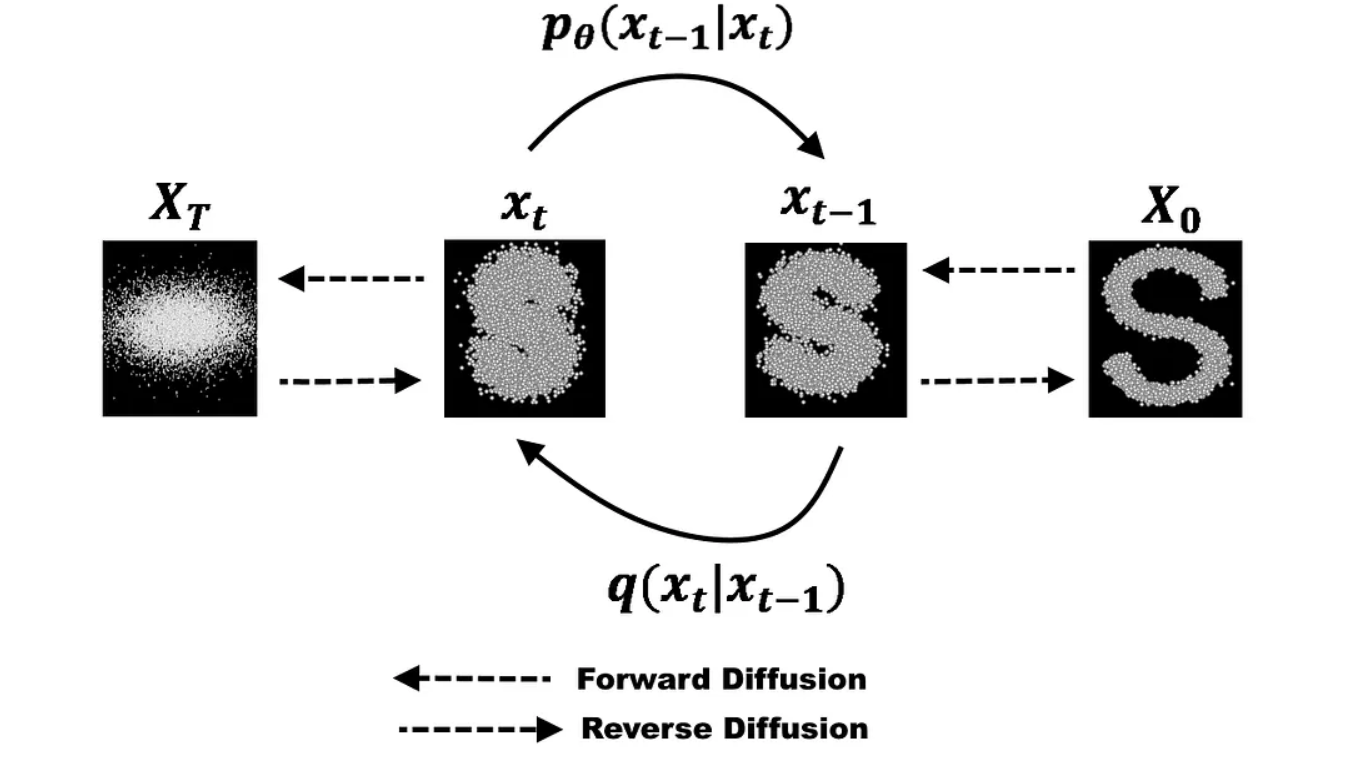
\includegraphics[width=12cm]{images_pfe/diffusion_process.png}
	\caption{Illustration des Processus de Diffusion : Forward Process et Reverse Process.}
	\label{fig:pro_diff}
\end{figure}
\FloatBarrier

Pour effectuer le débruitage, un réseau de neurones est utilisé. Ce réseau de
neurones est entraîné à détecter et à éliminer le bruit à chaque étape du
Reverse Process. Il apprend à prédire l'état précédent des données à partir de
l'état actuel bruité, permettant ainsi de reconstruire progressivement les
données originales. Cette méthode en deux phases, combinée à l'utilisation d'un
réseau de neurones [Figure \ref{fig:unet_}] pour le débruitage, permet de
modéliser et de générer des données synthétiques de haute qualité de manière
efficace et contrôlée.

\begin{figure}[hbt!]
	\centering
	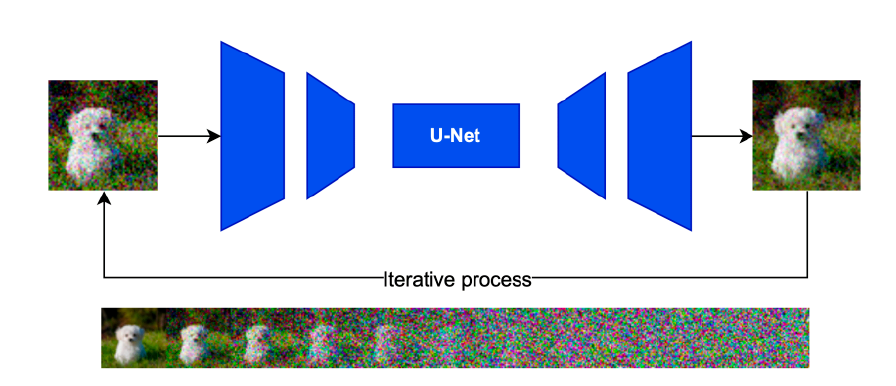
\includegraphics[width=12cm]{images_pfe/Unet.png}
	\caption{ Le processus d'entraînement d'un UNet pour prédire le bruit ajouté à l'image. [\cite{nichol2021improved}].}
	\label{fig:unet_}
\end{figure}
\FloatBarrier

\subsubsection{Forward Process (Bruitage)}

L'étape de bruitage ajoute progressivement du bruit gaussien aux données
réelles. Ce processus est modélisé comme une chaîne de Markov où chaque état \(
x_t \) dépend uniquement de l'état précédent \( x_{t-1} \).

La transition conditionnelle pour le bruitage est donnée par \ref{fig:bruitage}
:
\begin{equation}
	q(\mathbf{x}_t \mid \mathbf{x}_{t-1}) = \mathcal{N}(\mathbf{x}_t; \sqrt{1 - \beta_t} \mathbf{x}_{t-1}, \beta_t \mathbf{I})
	\label{fig:bruitage}
\end{equation}

où :
\begin{conditions}
	x_t & \text{état des données à l'étape \( t \)} \\
	\beta_t & \text{taux de bruitage (un hyperparamètre ou une fonction du temps)} \\
	\mathcal{N} & \text{distribution normale gaussienne} \\
	\mathbf{I} & \text{matrice identité}
\end{conditions}

La séquence complète des \( T \) étapes de bruitage est décrite par
\ref{equ:bruit_comp} :
\begin{equation}
	q(\mathbf{x}_{1:T} \mid \mathbf{x}_0) = \prod_{t=1}^T q(\mathbf{x}_t \mid \mathbf{x}_{t-1})
	\label{equ:bruit_comp}
\end{equation}

\textbf{Explication du Forward Process :}

\begin{itemize}
	\item À chaque étape \( t \), une petite quantité de bruit gaussien est ajoutée à \( x_{t-1} \), produisant \( x_t \).
	\item La moyenne de la distribution est \( \sqrt{1 - \beta_t} x_{t-1} \), indiquant
	      que la contribution des données d'origine diminue progressivement.
	\item La variance est \( \beta_t \), contrôlant la quantité de bruit ajouté.
\end{itemize}

\subsubsection{Reverse Process (Débruitage)}

L'étape de débruitage consiste à inverser le processus de bruitage pour
transformer le bruit gaussien en données réalistes. Cela se fait en utilisant
un modèle génératif pour approximer la distribution inverse.

La transition conditionnelle pour le débruitage est donnée par \ref{equ:debr}:

\begin{equation}
	p_\theta(\mathbf{x}_{t-1} \mid \mathbf{x}_t) = \mathcal{N}(\mathbf{x}_{t-1}; \mu_\theta(\mathbf{x}_t, t), \Sigma_\theta(\mathbf{x}_t, t))
	\label{equ:debr}
\end{equation}

où :
\begin{conditions}
	p_\theta & \text{distribution paramétrée par les poids du modèle \( \theta \)} \\
	\mu_\theta & \text{moyenne apprise par le modèle} \\
	\Sigma_\theta & \text{covariance apprise par le modèle}
\end{conditions}

\textbf{Explication du Reverse Process :}

\begin{itemize}
	\item Le modèle est entraîné pour prédire \( x_{t-1} \) à partir de \( x_t \).
	\item La moyenne \( \mu_\theta(x_t, t) \) est une fonction paramétrée par \( \theta
	      \), dépendant de \( x_t \) et du temps \( t \).
	\item La covariance \( \Sigma_\theta(x_t, t) \) représente l'incertitude du modèle.
\end{itemize}

\paragraph{Objectif d'Entraînement :}
L'objectif est de minimiser la divergence de Kullback-Leibler (KL) entre la
distribution réelle \( q \) et la distribution générée par le modèle \(
p_\theta \). La fonction de perte du modèle de diffusion est donnée par
l'équation \ref{equ:div_diff} :

\begin{equation}
	\mathcal{L} = \mathbb{E}_q \left[ \sum_{t=1}^T D_{KL}(q(\mathbf{x}_{t-1} \mid \mathbf{x}_t, \mathbf{x}_0) \| p_\theta(\mathbf{x}_{t-1} \mid \mathbf{x}_t)) \right]
	\label{equ:div_diff}
\end{equation}

\subsection{Applications des Modéles de Diffusion}
Les modèles de diffusion ont trouvé des applications dans divers domaines grâce
à leur capacité à générer des données synthétiques de haute qualité. Parmi les
applications remarquables des modèles de diffusion, on trouve:

\begin{itemize}
	\item \textbf{Génération d'images} : Les modèles de diffusion sont largement utilisés pour la génération d'images réalistes à partir de bruit aléatoire. Ils permettent de créer des images de haute qualité qui peuvent être utilisées dans le domaine de l'art, du design, et même dans la production de contenu multimédia.

	\item \textbf{Synthèse vocale} : Ces modèles sont également appliqués dans la génération de voix synthétiques, offrant des améliorations significatives dans la clarté et la naturalité de la voix produite, utilisée dans les assistants vocaux et les technologies de lecture automatique.

	\item \textbf{Création de vidéos} : En transformant des séquences de bruit en vidéos cohérentes, les modèles de diffusion peuvent générer des animations et des vidéos synthétiques, ouvrant de nouvelles possibilités dans le divertissement et la publicité.

	\item \textbf{Traitement et amélioration d'images} : Les modèles de diffusion peuvent être utilisés pour restaurer des images bruitées, améliorer la résolution des images, et effectuer des transformations d'image avancées telles que la colorisation et le changement de style.

	\item \textbf{Séries temporelles} : On peut aussi utiliser les modèles de diffusion pour d'autres types de données comme les séries temporelles. Ils peuvent aider à la prévision, à la détection d'anomalies et à la génération de nouvelles séries temporelles synthétiques [\cite{yang2023survey}].
\end{itemize}

Parmi les applications ayant connu un succès notable, on trouve :

\begin{itemize}
	\item \textbf{Stable Diffusion} : un modèle de diffusion qui a gagné en popularité pour sa capacité à générer des images d’une qualité exceptionnelle et son utilisation dans divers projets artistiques et commerciaux. Stable Diffusion est particulièrement apprécié pour sa flexibilité et sa robustesse, permettant aux artistes et aux créateurs de générer des œuvres d'art numériques impressionnantes avec un niveau de détail et de réalisme sans précédent. En outre, il est utilisé dans des industries telles que le design graphique, la publicité et même la production cinématographique, démontrant sa vaste applicabilité commerciale [\cite{rombach2022high}].

	\item \textbf{DALL-E de OpenAI} : Ce modèle est capable de créer des images à partir de descriptions textuelles [Figure \cite{fig:Dalle}], révolutionnant ainsi la manière dont nous concevons et interagissons avec les images générées par l’intelligence artificielle. DALL-E peut interpréter des descriptions textuelles complexes et générer des images correspondantes, ce qui ouvre de nouvelles possibilités en matière de création de contenu visuel. Par exemple, il peut créer des images de concepts ou d'objets inexistants basés uniquement sur des descriptions verbales, ce qui est extrêmement utile pour le prototypage, l'illustration de concepts et l'innovation créative. DALL-E a été salué pour sa capacité à comprendre et à visualiser des idées abstraites, rendant la technologie accessible et utile pour les designers, les artistes et les innovateurs.
\end{itemize}

\begin{figure}[hbt!]
	\centering
	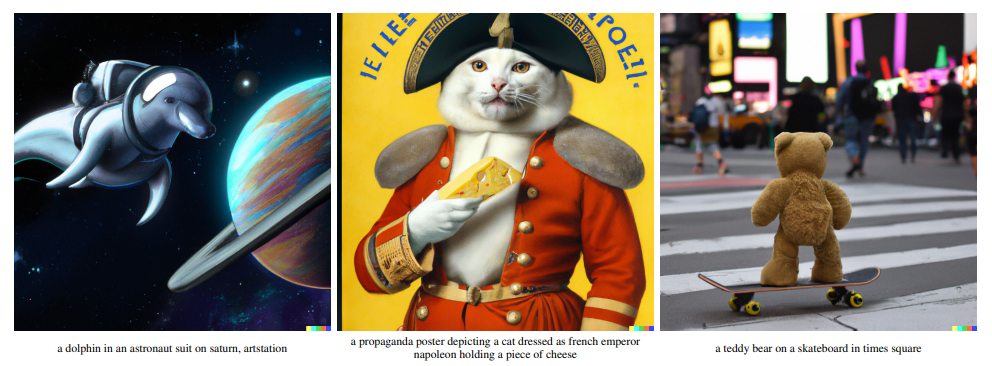
\includegraphics[width=12cm]{images_pfe/dalle.png}
	\caption{Exemple d’images générée par DALL-E2. [\cite{ramesh2022hierarchical}].}
	\label{fig:Dalle}
\end{figure}
\FloatBarrier

Ces applications démontrent la polyvalence et l'efficacité des modèles de
diffusion, faisant d'eux des outils indispensables dans l'arsenal de
l'intelligence artificielle moderne.

Les modèles de diffusion se sont révélés être une avancée remarquable dans le
domaine des modèles génératifs, en particulier pour leur capacité à produire
des données synthétiques de haute qualité, Leur robustesse, couplée à une
efficacité croissante, fait des modèles de diffusion un choix prometteur pour
de nombreuses applications en intelligence artificielle. Leur potentiel
continue de se déployer, suggérant une influence durable et croissante dans le
paysage de l'apprentissage automatique.

\section{Conclusion}
En conclusion, ce chapitre a présenté les modèles qui ont marqué un succès
significatif dans le domaine de l'intelligence artificielle générative. Nous
avons exploré trois des modèles les plus utilisés, à savoir les VAE
(Variational Autoencoders), les GANs (Generative Adversarial Networks) et les
modèles de diffusion. Chacun de ces modèles a été examiné en détail, tant en ce
qui concerne leur fonctionnement interne que leurs applications dans divers
domaines.

Les VAE se distinguent par leur capacité à apprendre des représentations
latentes continues, permettant une génération de données synthétiques avec une
grande cohérence. Les GANs, quant à eux, se sont imposés comme des outils
puissants pour générer des images réalistes, grâce à leur mécanisme
d'apprentissage par confrontation entre un générateur et un discriminateur.
Enfin, les modèles de diffusion, plus récents, offrent une approche unique pour
générer des données de haute qualité en partant de bruit et en débruitant
progressivement, rivalisant avec les techniques traditionnelles dans plusieurs
applications.

Ces trois modèles, bien que tous basés sur les réseaux de neurones et les
principes de la probabilité, diffèrent radicalement dans leur approche et leur
fonctionnement, ce qui leur confère des avantages spécifiques dans diverses
applications. Par ailleurs, d'autres modèles génératifs, tels que les grands
modèles de langage (Large Language Models) [\cite{attention_is_all_you_need}],
ont également montré un potentiel considérable, notamment dans la génération de
texte, et ils continuent d'évoluer rapidement.

Le domaine de l'intelligence artificielle générative est extrêmement dynamique
et en pleine expansion. Avec l'augmentation exponentielle des données
disponibles et l'accès croissant à des ressources de calcul puissantes, il est
certain que des innovations encore plus passionnantes émergeront dans un avenir
proche. Ce champ de recherche reste donc ouvert et prometteur, avec de
nombreuses opportunités pour de nouvelles découvertes et applications.

\newpage
%%%%%%%%%%%%%%%%%%%%%%%%%%%%%%%%%% Large Language Models%%%%%%%%%%%%%%%%%%%%%%%%%%%%%%%%%%%%ù

\chapter{Maintenance prédictive des moteurs électriques}
\section{Introduction}

La maintenance prédictive est devenue une approche incontournable pour la
gestion efficace des équipements industriels, en particulier les moteurs
électriques. Avec l'avènement de l'Industrie 4.0 et l'intégration croissante de
l'Internet des Objets (IoT) et de l'intelligence artificielle (IA) dans les
processus industriels[\cite{dalenogare2018industry4}], la maintenance
prédictive permet d'anticiper les défaillances potentielles avant qu'elles ne
se produisent, assurant ainsi une continuité opérationnelle optimale et une
réduction significative des coûts de maintenance [\cite{Mrozek2023}].

Les moteurs électriques, étant au cœur de nombreuses applications
industrielles, représentent des composants critiques dont la fiabilité et
l'efficacité doivent être constamment surveillées. La maintenance prédictive
pour ces moteurs repose sur l'analyse en temps réel de diverses données
opérationnelles telles que les vibrations, les températures, les courants
électriques et les niveaux de bruit. Grâce à des capteurs avancés et à des
algorithmes sophistiqués, il est possible de détecter des anomalies subtiles et
d'identifier les signes précurseurs de défaillances mécaniques ou électriques
[\cite{Bentivogli2023}].

L'adoption de la maintenance prédictive apporte plusieurs avantages majeurs.
Elle permet non seulement d'améliorer la durée de vie des moteurs électriques,
mais aussi de planifier les interventions de maintenance de manière plus
stratégique, évitant ainsi les arrêts imprévus et minimisant les perturbations
de la production. De plus, cette approche contribue à une gestion plus durable
des ressources en réduisant les déchets et en optimisant l'utilisation de
l'énergie.

Dans ce chapitre, nous explorerons en détail les principes fondamentaux de la
maintenance prédictive appliquée aux moteurs électriques. Nous examinerons les
technologies et outils utilisés pour la collecte et l'analyse des données,
ainsi que les différentes méthodes d'interprétation des signaux pour prévoir
les défaillances. Enfin, nous discuterons des défis et des perspectives
d'avenir de cette approche, mettant en lumière son rôle crucial dans la
transformation numérique de l'industrie.

\section{Types de Maintenance}

\subsection{Maintenance Corrective}
La maintenance corrective est réalisée après la détection d’une panne ou d’une
défaillance. Son objectif est de remettre l’équipement en état de fonctionner
en corrigeant le défaut[\cite{Sezdi2019}].

La maintenance corrective intervient généralement après l'échec de
l'équipement, lorsque celui-ci cesse de fonctionner comme prévu. Elle est
souvent utilisée dans les industries où le coût de l'arrêt non planifié est
moins critique ou où les équipements ne peuvent pas être surveillés en continu.
Par exemple, dans certaines installations de production manufacturière, les
interventions correctives peuvent être tolérées si les pièces de rechange sont
facilement disponibles et si les réparations peuvent être effectuées
rapidement. Cette méthode est également courante dans les petites entreprises
où les ressources pour une maintenance plus proactive peuvent être limitées.

\subsection{Maintenance Préventive}
La maintenance préventive est effectuée régulièrement selon un calendrier
prédéfini ou en fonction du temps ou du nombre de cycles d’utilisation,
indépendamment de l’état de l’équipement. Elle vise à réduire la probabilité de
défaillance [\cite{Sezdi2019}].

La maintenance préventive repose sur des inspections et des services réguliers
pour éviter les pannes inattendues. Cette méthode est largement adoptée dans
les industries telles que l'aérospatiale, l'automobile et les centrales
électriques où la fiabilité et la sécurité sont critiques. Par exemple, dans
l'industrie aéronautique, les avions subissent des inspections régulières et
des entretiens programmés pour garantir la sécurité des vols et prévenir les
pannes en vol. De même, dans les centrales électriques, des programmes de
maintenance préventive stricts sont mis en place pour assurer un fonctionnement
continu et sûr des générateurs et des turbines.

\subsection{Maintenance Prédictive}
La maintenance prédictive repose sur la surveillance en temps réel et l’analyse
des données de l’équipement pour anticiper les pannes avant qu’elles ne
surviennent. Elle utilise des techniques telles que la vibration, l’analyse
d’huile, l’imagerie thermique, et les données de performance​
[\cite{Bentivogli2023, Sangeetha2017}].

La maintenance prédictive vise à identifier les signes avant-coureurs de
défaillances potentielles en utilisant des technologies avancées. Les capteurs
IoT, les analyses de données et les algorithmes d'apprentissage automatique
sont employés pour surveiller les conditions des équipements en temps réel.
Cette approche est particulièrement utile dans les industries telles que le
pétrole et le gaz, la production d'énergie et la fabrication de haute
précision. Par exemple, dans les centrales éoliennes, les systèmes de
maintenance prédictive surveillent les vibrations et les températures des
composants critiques pour prévenir les pannes coûteuses et prolonger la durée
de vie des équipements. Dans l'industrie manufacturière, elle permet de
maintenir la qualité des produits et d'optimiser les cycles de production en
réduisant les temps d'arrêt imprévus.

Ces trois types de maintenance, que sont la maintenance prédictive, corrective
et préventive, ont chacun leurs avantages et inconvénients. Nous présentons les
avantages et inconvénients de chaque technique dans le tableau
\ref{tab:comparaison-maintenance}. De plus, nous présentons la figure
\ref{fig:pred} pour illustrer l'ordre chronologique à suivre pour effectuer la
maintenance.

\begin{figure}[hbt!]
	\centering
	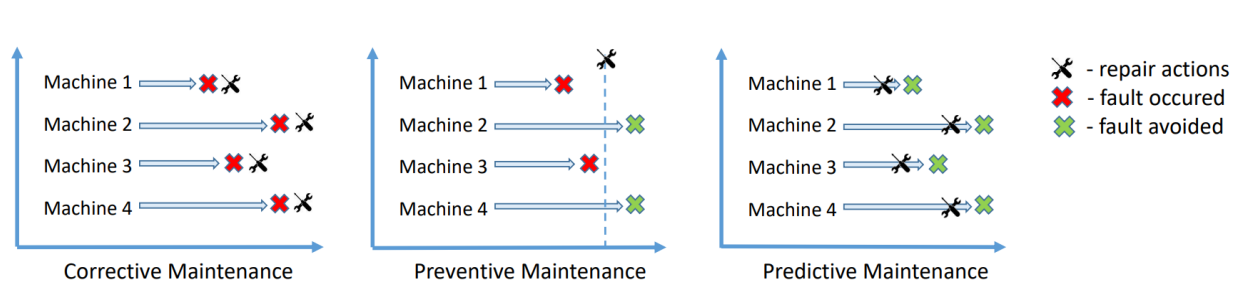
\includegraphics[width=18cm]{images_pfe/predictive.png}
	\caption{Stratégies de maintenance montrant les différentes étapes du processus de réparation avant et après la défaillance potentielle de l'équipement. [\cite{Mrozek2023}].}
	\label{fig:pred}
\end{figure}
\FloatBarrier

\begin{table}[h]
	\centering
	\begin{tabular}{|l|p{5cm}|p{5cm}|}
		\hline
		\textbf{Type de Maintenance} & \textbf{Avantages}                                                                                                                                            & \textbf{Inconvénients}                                                                                                                   \\
		\hline
		\textbf{Corrective}          & Simple à planifier, nécessite moins de surveillance continue                                                                                                  & Arrêts imprévus, coûts élevés de réparation d’urgence, et perturbations importantes de la production                                     \\
		\hline
		\textbf{Préventive}          & Réduit les risques de pannes imprévues, améliore la fiabilité de l’équipement                                                                                 & Coûts supplémentaires en raison de l’entretien d’équipements encore en bon état, nécessite une planification rigoureuse                  \\
		\hline
		\textbf{Prédictive}          & Permet de planifier les interventions de manière optimale, minimise les arrêts non planifiés, prolonge la durée de vie des équipements, et optimise les coûts & Nécessite des investissements initiaux en capteurs et en technologie de surveillance, ainsi que des compétences analytiques spécialisées \\
		\hline
	\end{tabular}
	\caption{Comparaison entre les Types de Maintenance}
	\label{tab:comparaison-maintenance}
\end{table}

\section{Maintenance prédictive pour les  moteurs électriques }

La maintenance prédictive des moteurs électriques est une approche proactive
qui vise à anticiper les pannes et à optimiser la performance des équipements.
Contrairement à la maintenance corrective, qui intervient après la survenue
d'un problème, ou à la maintenance préventive, qui suit un calendrier fixe, la
maintenance prédictive s'appuie sur la surveillance continue de l'état des
machines et l'analyse de données en temps réel.

Cette stratégie utilise des technologies avancées telles que l'Internet des
objets (IoT), l'intelligence artificielle (IA) et l'analyse de données pour
collecter et interpréter des informations sur les vibrations, la température,
le courant et d'autres paramètres opérationnels des moteurs électriques. Grâce
à ces données, il est possible de détecter les signes avant-coureurs de
défaillances potentielles, comme l'usure des roulements, les déséquilibres de
rotor ou les problèmes d'isolation.

L'objectif principal de la maintenance prédictive est d'améliorer la fiabilité
et la durée de vie des moteurs électriques tout en réduisant les coûts de
maintenance et les interruptions de service. En anticipant les problèmes avant
qu'ils ne deviennent critiques, les entreprises peuvent planifier les
interventions de maintenance de manière plus efficace, minimisant ainsi les
temps d'arrêt imprévus et les coûts associés.

\subsection{Moteurs électriques}

Les moteurs électriques sont des dispositifs essentiels qui convertissent
l'énergie électrique en énergie mécanique, jouant un rôle crucial dans de
nombreux aspects de la vie quotidienne et industrielle. Utilisés dans divers
secteurs tels que la fabrication, le transport et les applications domestiques,
les moteurs électriques permettent un contrôle précis, indispensable pour les
applications industrielles nécessitant une régulation rigoureuse de la vitesse
et du couple.

Parmi les différents types de moteurs électriques, les moteurs asynchrones, ou
moteurs à induction, occupent une place prépondérante. Inventés par Nikola
Tesla, ces moteurs sont largement utilisés en raison de leur simplicité, de
leur robustesse et de leur coût relativement bas. Un moteur asynchrone
fonctionne sur le principe de l'induction électromagnétique : lorsqu'un courant
alternatif traverse les bobines du stator, un champ magnétique tournant est
créé, induisant un courant dans le rotor. Ce courant induit génère à son tour
un champ magnétique qui interagit avec celui du stator, produisant un couple
qui fait tourner le rotor.

Ces moteurs sont utilisés dans une vaste gamme d'industries et d'applications.
Dans l'industrie manufacturière, ils entraînent des convoyeurs, des broyeurs et
des compresseurs. Dans les systèmes de traction, ils sont essentiels pour les
trains et les véhicules électriques. De plus, dans les services publics, ils
sont utilisés pour les pompes, les ventilateurs et les systèmes de ventilation
et de climatisation. Les moteurs asynchrones se distinguent par leur fiabilité,
leur capacité à fonctionner dans des conditions difficiles et leur maintenance
relativement facile, ce qui en fait un choix privilégié pour de nombreuses
applications industrielles et domestiques.

\subsubsection{Moteurs Asynchrones}

Il existe deux types de moteurs asynchrones : monophasés et triphasés. Dans
cette section, nous aborderons spécifiquement les moteurs triphas, la figure
\ref{fig:moteur-asynchrone} illustre les principaux composants d'un moteur
asynchrone triphasé, également appelé machine à induction:

\begin{figure}[hbt!]
	\centering
	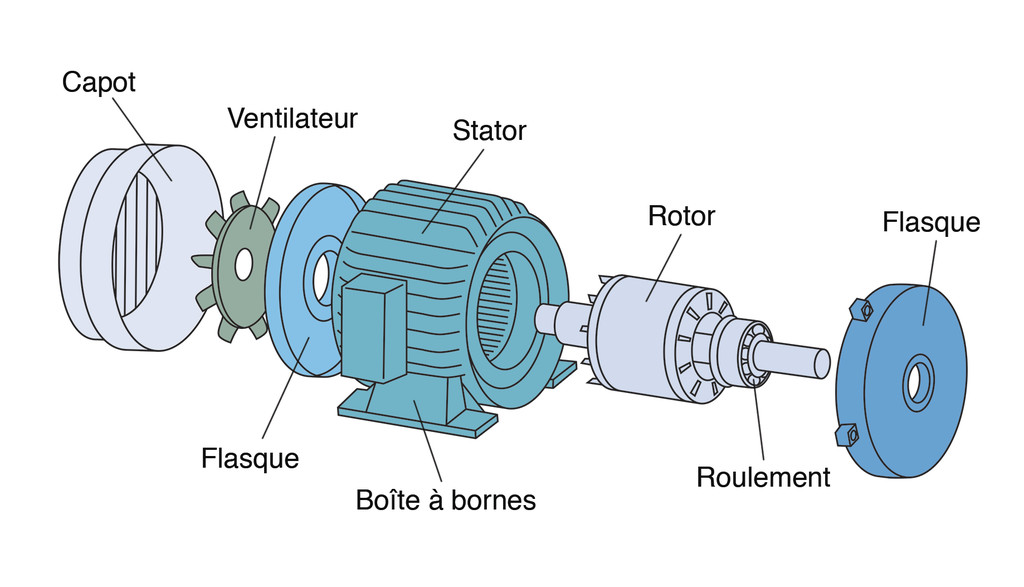
\includegraphics[width=12cm]{images_pfe/motor.jpg}
	\caption{
		Principaux Composants d'un moteur asynchrone triphasé (Machine à Induction).}
	\label{fig:moteur-asynchrone}
\end{figure}
\FloatBarrier

\begin{itemize}
	\item \textbf{Capot} : Il s'agit de la couverture externe du moteur qui protège les composants internes de la poussière, de l'humidité et d'autres contaminants.
	\item \textbf{Ventilateur} : Situé à côté du capot, le ventilateur assure la ventilation du moteur en refroidissant les composants internes pour éviter la surchauffe.
	\item \textbf{Flasque} : Les flasques sont des plaques situées aux extrémités du moteur, qui maintiennent les autres composants en place et assurent l'alignement correct de l'axe du rotor.
	\item \textbf{Stator} : C'est la partie fixe du moteur. Il est constitué de bobines de fil de cuivre qui génèrent un champ magnétique rotatif lorsque le courant triphasé y circule.
	\item \textbf{Boîte à bornes} : Située sur le stator, elle abrite les connexions électriques du moteur, permettant de connecter le moteur à l'alimentation électrique.
	\item \textbf{Rotor} : C'est la partie rotative du moteur qui tourne sous l'effet du champ magnétique généré par le stator. Il est connecté à l'axe et transfère l'énergie mécanique.
	\item \textbf{Roulement} : Les roulements soutiennent le rotor et permettent son mouvement rotatif en minimisant la friction.
\end{itemize}

\subsubsection{Défauts des Moteurs Asynchrones}

Les moteurs asynchrones peuvent présenter divers défauts mécaniques et
électriques. Ces défauts peuvent affecter les performances et la durée de vie
du moteur. Dans les paragraphes qui suivent, nous allons examiner en détail ces
défauts.

\paragraph{Défauts Mécaniques} : Deux défauts mécaniques se manifestent fréquemment dans les moteurs asynchrones :

\subparagraph{Défaut d'excentricité de l'entrefer}:
L'excentricité de l'entrefer se produit lorsque l'espace entre le stator et le
rotor n'est pas uniforme. Cela peut être causé par un désalignement, une usure
inégale des roulements ou des défauts de fabrication. Ce défaut peut entraîner
des vibrations excessives, des bruits anormaux et une usure prématurée des
composants du moteur.

\subparagraph{Dommages aux roulements}:
Les roulements sont essentiels pour le bon fonctionnement du rotor. Les
dommages aux roulements peuvent être causés par une lubrification insuffisante,
des contaminants, une surcharge ou une mauvaise installation. Les symptômes de
dommages aux roulements incluent des vibrations élevées, des bruits de
grincement ou de cliquetis, et une augmentation de la température de
fonctionnement.

\paragraph{Défauts Électriques} : Les moteurs asynchrones présentent souvent deux types de défauts électriques:

\subparagraph{Court-circuit entre spires}:
Un court-circuit entre spires se produit lorsque l'isolation entre les
enroulements d'une bobine du stator est endommagée, permettant au courant de
circuler directement entre les spires. Ce défaut peut entraîner une surchauffe
localisée, une diminution de l'efficacité du moteur et, dans les cas graves,
une défaillance complète du moteur.

\subparagraph{Barre de rotor cassée}:
Les barres de rotor sont des composants clés du rotor de la cage d'écureuil
dans un moteur asynchrone. Une barre de rotor cassée peut se produire en raison
de contraintes mécaniques répétées, de surcharges ou de défauts de fabrication.
Ce défaut peut provoquer un déséquilibre du rotor, des vibrations excessives et
une diminution des performances du moteur.

%%%%%%%%%%%%%%%%%%%%%Traitement de Signal%%%%%%%%%%%%%%%%%%%%%ùù

\section{Traitement de Signal Pour les moteurs électriques}

Un signal est une représentation physique ou une mesure de certaines
caractéristiques d’un système, généralement en fonction du temps. Dans le
contexte des moteurs électriques, les signaux peuvent inclure des courants, des
tensions, des vitesses de rotation, des températures, des vibrations, et bien
d'autres paramètres. Ces signaux peuvent être capturés par des capteurs
installés sur ou à proximité du moteur.

L'analyse des signaux de courant et de tension de sortie est cruciale pour la
maintenance prédictive des moteurs électriques. Des techniques telles que
l'analyse des harmoniques, l'analyse du spectre de fréquence et la surveillance
des formes d'onde permettent de détecter les anomalies et de diagnostiquer les
défauts avant qu'ils ne causent des pannes majeures. Par exemple, un
déséquilibre dans les courants de phase peut indiquer un défaut mécanique comme
une excentricité de l'entrefer, tandis qu'une augmentation des harmoniques peut
signaler un court-circuit entre spires.

\subsection{Signaux Triphasés dans les Moteurs Électriques}

Les moteurs électriques triphasés utilisent des signaux électriques triphasés
[Figure \ref{fig:moteur-asynchrone-tri}] pour fonctionner efficacement. Ces
signaux, qui consistent en trois courants alternatifs déphasés de 120 degrés
chacun, sont essentiels pour la création d'un champ magnétique rotatif dans le
stator, qui à son tour entraîne la rotation du rotor.

\subsubsection*{Signaux d'entrée}

Les signaux d'entrée d'un moteur électrique triphasé sont constitués de
courants et de tensions triphasés. Chaque phase est décalée de 120 degrés par
rapport aux autres, permettant une distribution équilibrée de la puissance et
réduisant les vibrations et les pertes. Les courants et tensions triphasés
d'entrée doivent être équilibrés et stables pour assurer un fonctionnement
optimal du moteur. Des déséquilibres ou des variations peuvent indiquer des
problèmes dans l'alimentation ou des défauts internes.

\subsubsection*{Signaux de sortie}

Les signaux de sortie d'un moteur électrique, principalement les courants et
les tensions mesurés aux bornes du moteur, peuvent fournir des informations
précieuses sur l'état de santé du moteur. Un moteur en bon état génère des
signaux de sortie avec un certain motif ou "pattern" caractéristique. Ce motif
est souvent analysé en termes de formes d'onde, d'harmoniques et de spectres de
fréquence.

\begin{figure}[hbt!]
	\centering
	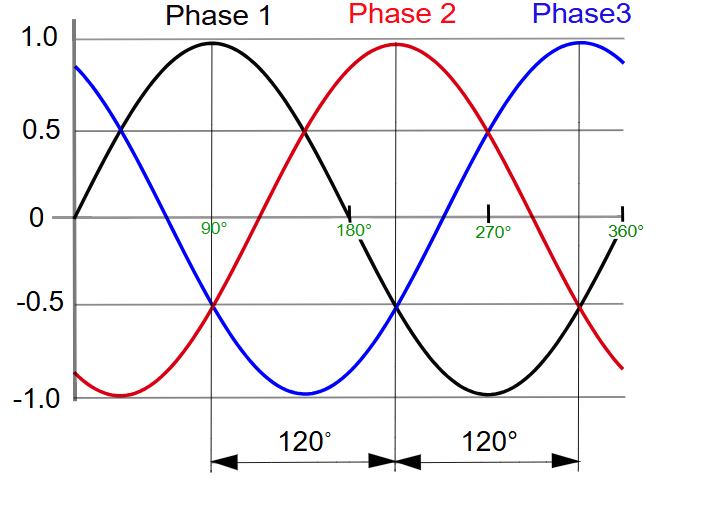
\includegraphics[width=12cm]{images_pfe/triphase.png}
	\caption{
		Signaux électriques triphasés.}
	\label{fig:moteur-asynchrone-tri}
\end{figure}
\FloatBarrier

\subsection{Motor Current Signature Analysis (MCSA)}

L'analyse des signaux de courant et de tension de sortie est cruciale pour la
maintenance prédictive des moteurs électriques. Une technique particulièrement
efficace pour cette analyse est la Motor Current Signature Analysis (MCSA).

La MCSA est une méthode de surveillance et de diagnostic basée sur l'analyse
des courants du moteur. En mesurant et en analysant les signatures de courant,
il est possible de détecter des défauts internes et externes du moteur
	[\cite{bonetjara2023sensorless}]. La MCSA peut identifier des problèmes tels
que :
\begin{itemize}
	\item \textbf{Défauts mécaniques} : Excentricité de l'entrefer, désalignement, déséquilibre.
	\item \textbf{Défauts électriques} : Court-circuit entre spires, barres de rotor cassées, défauts d'isolation.
	\item \textbf{Problèmes d'alimentation} : Déséquilibre de phase, distorsions harmoniques.
\end{itemize}

La MCSA utilise des techniques d'analyse de spectre de fréquence pour
identifier les composantes spécifiques du signal de courant qui sont associées
à différents types de défauts. Par exemple, un déséquilibre du rotor peut
générer des fréquences spécifiques qui apparaissent dans le spectre de courant.
En détectant ces fréquences, il est possible de diagnostiquer le défaut avant
qu'il ne cause une panne majeure.

\subsubsection*{Avantages de la MCSA}

L'utilisation de la MCSA pour la surveillance des moteurs électriques présente
plusieurs avantages :
\begin{itemize}
	\item \textbf{Détection précoce des défauts} : Identification des problèmes avant qu'ils ne deviennent critiques.
	\item \textbf{Maintenance proactive} : Planification des interventions de maintenance basées sur l'état réel du moteur.
	\item \textbf{Réduction des coûts} : Minimisation des temps d'arrêt imprévus et des réparations coûteuses,
	      elle ne nécessite pas de capteurs externes comme ceux de température et de vibration.
	\item \textbf{Amélioration de la fiabilité} : Augmentation de la durée de vie des moteurs et amélioration de leur performance globale.
\end{itemize}

la surveillance continue des signaux triphasés et l'utilisation de techniques
comme la MCSA sont essentielles pour assurer le bon fonctionnement et la
longévité des moteurs électriques. L'analyse proactive des courants et des
tensions permet de détecter les problèmes potentiels à un stade précoce,
facilitant ainsi une intervention rapide et réduisant les coûts de maintenance.

\subsection{Transformée de Fourier Rapide (FFT)}

La Transformée de Fourier Rapide (FFT pour Fast Fourier Transform ) est un
algorithme essentiel dans le traitement des signaux, utilisé pour transformer
un signal du domaine temporel au domaine fréquentiel. Le principe fondamental
de la FFT repose sur la décomposition d'un signal complexe en une somme de
sinusoïdes, chacune correspondant à une fréquence spécifique et une amplitude
déterminée. Cette capacité à révéler les composantes fréquentielles d'un signal
en fait un outil crucial pour l'analyse, la filtration et la compression des
données dans diverses applications scientifiques et industrielles
	[\cite{duhamel_vetterli_1989}].

Par exemple, si l'on possède un signal dans le domaine temporel, on peut le
transformer et le visualiser dans le domaine fréquentiel en utilisant la
Transformée de Fourier Rapide (FFT) [Figure \ref{fig:fft}]. Cette
transformation permet de représenter les composantes en fréquence du signal, ce
qui est fondamental pour comprendre sa structure spectrale.

La FFT est basée sur l'équation suivante \ref{equ:fft}:

\begin{equation}
	X(k) = \sum_{n=0}^{N-1} x(n) \cdot e^{-j \cdot 2\pi \cdot k \cdot n / N}
	\label{equ:fft}
\end{equation}

Où :
\begin{conditions}
	X(k) & représente l'amplitude de la fréquence \( k \) \\
	x(n) & est la valeur du signal à l'instant \( n \) \\
	N & est le nombre total d'échantillons du signal \\
	j & est l'unité imaginaire
\end{conditions}

Cette équation permet de calculer les composantes fréquentielles $X(k)$ pour
chaque fréquence $k$, transformant ainsi le signal du domaine temporel vers le
domaine fréquentiel.

\begin{figure}[hbt!]
	\centering
	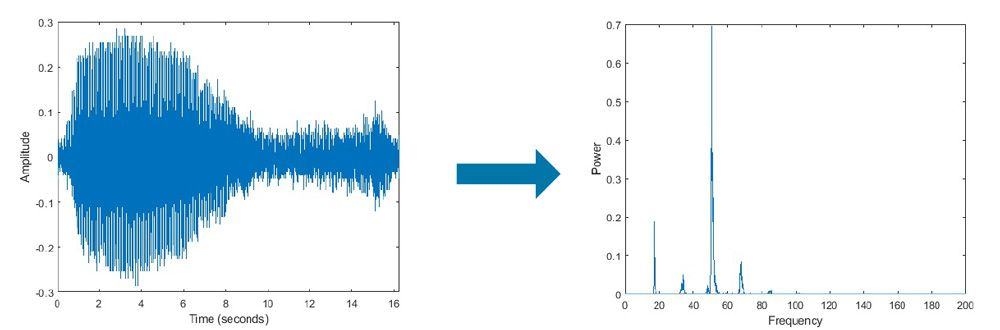
\includegraphics[width=14cm]{images_pfe/fft.jpg}
	\caption{
		Exemple de transformation d'un signal du domaine temporel au domaine fréquentiel à l'aide de la FFT.}
	\label{fig:fft}
\end{figure}
\FloatBarrier

\subsection*{Importance de la FFT dans l'Analyse des Signaux}

\begin{enumerate}
	\item \textbf{Identification des Fréquences Dominantes} : La FFT permet de décomposer un signal complexe en ses différentes composantes fréquentielles. Cette décomposition est cruciale pour identifier les fréquences dominantes dans un signal, ce qui est essentiel dans des domaines comme la détection de pannes en ingénierie ou l'analyse du spectre audio.

	\item \textbf{Filtrage et Traitement des Signaux} : En permettant de travailler dans le domaine fréquentiel, la FFT facilite la conception de filtres numériques qui peuvent extraire ou supprimer des fréquences spécifiques d'un signal, améliorant ainsi la qualité du signal ou isolant des caractéristiques particulières.

	\item \textbf{Compression de Données} : La FFT est également utilisée dans des techniques de compression, telles que la compression d'image (JPEG) ou audio (MP3), où elle permet de réduire la quantité de données nécessaires pour représenter un signal tout en conservant ses caractéristiques essentielles.
\end{enumerate}

Dans le domaine des moteurs électriques, l'analyse fréquentielle des signaux
est particulièrement cruciale. Les moteurs électriques sont soumis à diverses
conditions de fonctionnement qui peuvent entraîner des défauts ou des
dysfonctionnements. L'analyse par FFT des signaux de courant, de tension ou de
vibration provenant de ces moteurs permet d'identifier les composantes
fréquentielles associées à ces anomalies. Par exemple, la présence de
fréquences spécifiques dans le spectre peut indiquer des problèmes tels que le
déséquilibre, le désalignement, les défauts de roulements ou les
courts-circuits dans les enroulements.

\section{Donneés: Séries Temporelles}

Dans de nombreux contextes, les données de séries temporelles peuvent être
considérées comme des signaux, en particulier lorsque les points de données
représentent des mesures prises à intervalles de temps réguliers. Par exemple,
les relevés de température quotidienne constituent une série temporelle qui
peut être analysée comme un signal pour identifier les schémas, les tendances
et les anomalies [\cite{brophy2023gan}] . Il existe deux types de séries
temporelles : discrètes et continues [Figure \ref{fig:time-series}].

Les séries temporelles discrètes, caractérisées par des points de données
espacés à des intervalles réguliers, sont couramment utilisées dans de
nombreuses disciplines pour faciliter l'analyse statistique et la prévision.
Elles permettent une compréhension claire des tendances à long terme et des
variations saisonnières, et sont particulièrement utiles dans des domaines tels
que la climatologie, l'économie et les sciences sociales [\cite{brophy2023gan}]
.

À l'opposé, les séries temporelles continues, où les données sont collectées à des
intervalles infinitésimaux, offrent une représentation plus détaillée et précise des
phénomènes étudiés. Cette approche est cruciale dans des domaines tels que le traitement
du signal, la physique et l'ingénierie, où une résolution temporelle fine est nécessaire
pour capturer les dynamiques rapides et les variations subtiles des systèmes [\cite{brophy2023gan}].

\begin{figure}[hbt!]
	\centering
	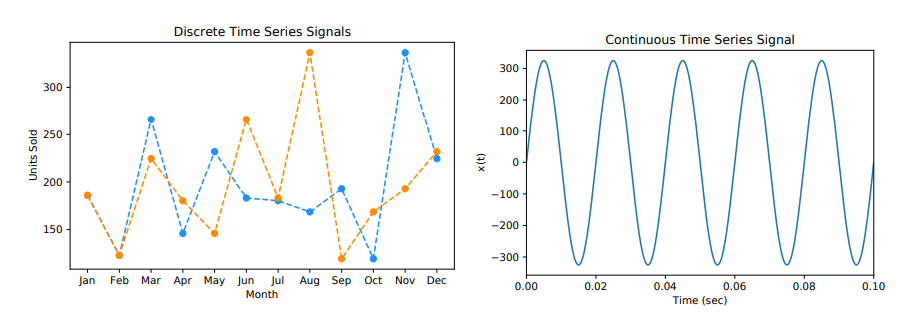
\includegraphics[width=12cm]{images_pfe/timeseries.png}
	\caption{
		Exemples de tracés de séries temporelles discrètes (à gauche) et continues (à droite) [\cite{brophy2023gan}] .}
	\label{fig:time-series}
\end{figure}
\FloatBarrier

\subsubsection{Catégories de Séries Temporelles}

Il existe deux catégories de séries temporelles : univariée et
multivariée[\cite{fawaz2019deep}].

\textbf{Définition 1: Série temporelle univariée}

Une série temporelle univariée $X$ est un ensemble ordonné de valeurs réelles.
La longueur de $X$ est égale au nombre de valeurs réelles $T$:

\begin{equation}
	X = [x_1, x_2, \ldots, x_T]
\end{equation}

où $x_i \in \mathbb{R}$ et $i = 1, 2, \ldots, T$.

Par exemple, une série temporelle univariée de température prise toutes les
heures pendant une journée pourrait être représentée par : $X = [15.5, 16.0,
	16.5, \ldots, 20.0]$, où $T = 24$.

\textbf{Définition 2: Série temporelle multivariée}

Une série temporelle multivariée de dimension $M$, notée $X$, se compose de $M$
séries temporelles univariées différentes, chaque $X_i$ étant un vecteur de
$\mathbb{R}^T$:

\begin{equation}
	X = [X_1, X_2, \ldots, X_M]
\end{equation}

où $X_i = [x_{i1}, x_{i2}, \ldots, x_{iT}]$, avec $x_{ij} \in \mathbb{R}$ pour
$i = 1, 2, \ldots, M$ et $j = 1, 2, \ldots, T$.

Par exemple, une série temporelle multivariée de dimension $M=2$, comprenant la
température et l'humidité relevées toutes les heures pendant une journée,
pourrait être représentée par : $X = [X_1, X_2]$, où $X_1$ représente la
température et $X_2$ représente l'humidité, chacun avec $T = 24$.

\section{Conclusion}

La maintenance prédictive des moteurs électriques représente une avancée
significative dans la gestion des actifs industriels, offrant une approche
proactive qui vise à anticiper les pannes et à optimiser la performance des
équipements. Contrairement à la maintenance corrective, qui intervient après la
survenue d’un problème, et à la maintenance préventive, qui suit un calendrier
fixe, la maintenance prédictive repose sur la surveillance continue de l’état
des machines et l’analyse de données en temps réel.

Cette stratégie utilise des technologies avancées telles que l'Internet des
objets (IoT), l'intelligence artificielle (IA) et l'analyse de données pour
collecter et interpréter des informations critiques sur les moteurs
électriques, permettant ainsi de détecter les signes avant-coureurs de
défaillances potentielles. L’objectif principal de cette approche est
d’améliorer la fiabilité et la durée de vie des moteurs électriques tout en
réduisant les coûts de maintenance et les interruptions de service.

En intégrant des techniques telles que l'analyse de la signature du courant
moteur (MCSA) à la maintenance prédictive, et en utilisant la transformation de
Fourier rapide (FFT), nous pouvons détecter précocement les défauts en analysant les
courants électriques du moteur. Cette approche combinée simplifie la
maintenance, optimise les coûts et élimine la nécessité de capteurs externes.

Enfin, l'analyse des séries temporelles, qu'elles soient discrètes ou
continues, joue un rôle crucial dans ce processus en fournissant des données
détaillées et précises pour l'analyse des signaux et l'identification des
anomalies. La distinction entre séries temporelles univariées et multivariées
enrichit encore cette approche, permettant une analyse plus complète et
intégrée des différentes variables opérationnelles.

